\documentclass[pdf,ps,8pt]{beamer}

\usepackage{lmodern}
\usepackage{amsmath}
\usepackage{color}
\usepackage{bbold}
\usepackage{cancel}
\usepackage{slashed}
\usepackage{graphicx}
\usepackage{verbatim}
\usepackage{textcomp}

\usetheme{Singapore}

\definecolor{palegray}{rgb}{0.82,0.822,0.82}
\newcommand{\preliminary}{
{ \rput{30}(7,-4.0){\fontsize{40}{40}\selectfont {\color{palegray}Preliminary Preliminary}} }
}

\newcommand{\textapprox}{\raisebox{0.5ex}{\texttildelow}}

\newcommand{\miniscule}{\fontsize{3pt}{4pt}\selectfont}

\def\MSbar{$\overline{\mathrm{MS}}$}
\def\gev{\,\mathrm{GeV}}
\def\mev{\,\mathrm{MeV}}
\def\fm{\,\mathrm{fm}}
\def\SU{\mathrm{SU}}
\def\su#1#2{\SU(#1)_\mathrm{#2}}
\def\rpisq{\langle r_\pi^2\rangle}
% final values
\def\rpisqsim{0.38(4)}  % pole fit for 330 MeV pion
\def\rpisqsu2sim{0.354(31)}  % su2 fit for 330 MeV pion
\def\rpisqsimlong{0.382(42)}
\def\rpisqphys{0.418(31)} % SU(2) chi extrap
\def\rpisqphyslong{0.418(31)}
\def\lsixr{-0.0093(10)} % SU(2)
\def\Lniner{0.0031(6)}  % SU(3)

\newcommand{\chpt}{\chi^{\rm PT}}
\newcommand{\tchpt}{$\chi^{\rm PT}$}
\newcommand{\tchptthree}{$\chi^{\rm PT}_3$}
\newcommand{\tchpttwo}{$\chi^{\rm PT}_2$}

\newcommand{\xiav}{\langle\,\xi\,\rangle}
\newcommand{\xisqav}{\langle\,\xi^2\,\rangle}


\newcommand{\mD}{\left(\begin{array}{cc} \DO & \Dd \\  \Ddb&\DOb \end{array} \right)}

\newcommand{\Ob}{\bar{\Omega}}

\newcommand{\DO}{D_\Omega}
\newcommand{\Dd}{D_\partial}
\newcommand{\DOi}{D_\Omega^{-1}}
\newcommand{\DOid}{D_\Omega^{-\dagger}}
\newcommand{\Pd} {\mathbb{P}_\partial}
\newcommand{\PO} {\mathbb{P}_\Omega}

\newcommand{\DOb}{D_{\bar{\Omega}}}
\newcommand{\Ddb}{D_{\bar{\partial}}}
\newcommand{\DObi}{D_{\bar{\Omega}}^{-1}}
\newcommand{\DObid}{D_{\bar{\Omega}}^{-\dagger}}
\newcommand{\Pdb}{\mathbb{P}_{\bar{\partial}}}
\newcommand{\POb} {\mathbb{P}_{\bar\Omega}}

\newcommand{\Phidb}{\mathbb{\phi}_{\bar{\partial}}}
\newcommand{\etadb}{\mathbb{\eta}_{\bar{\partial}}}

\newcommand{\hDO}{\hat D_\Omega}
\newcommand{\hDd}{\hat D_\partial}
\newcommand{\hDOi}{\hat D_\Omega^{-1}}
\newcommand{\hPd} {\hat{\mathbb{P}}_\partial}

\newcommand{\hDOb}{\hat D_{\bar{\Omega}}}
\newcommand{\hDdb}{\hat D_{\bar{\partial}}}
\newcommand{\hDObi}{\hat D_{\bar{\Omega}}^{-1}}
\newcommand{\hPdb}{\hat{\mathbb{P}}_{\bar{\partial}}}

\newcommand{\mul}[1]{\left(\begin{array}{cc}#1 & 0 \\ 0& 0\end{array}\right)}
\newcommand{\mur}[1]{\left(\begin{array}{cc}0  & #1\\ 0& 0\end{array}\right)}
\newcommand{\mll}[1]{\left(\begin{array}{cc}0  & 0 \\ #1 & 0\end{array}\right)}
\newcommand{\mlr}[1]{\left(\begin{array}{cc}0  & 0 \\ 0& #1\end{array}\right)}

\newcommand{\mDO}{\mul{ \DO}}
\newcommand{\mDd}{\mur{ \Dd}}
\newcommand{\mDOi}{\mul{\DOi}}
\newcommand{\mPd} {\mlr{\Pd}}

\newcommand{\mDOb}{\mlr{\DOb}}
\newcommand{\mDdb}{\mll{\Ddb}}
\newcommand{\mDObi}{\mlr{\DObi}}
\newcommand{\mPdb}{\mul{\Pdb}}
\newcommand{\rmod}{\mathrm{mod}}
\newcommand{\rdiv}{\mathrm{div}}

\newcommand{\link}[1]{\href{#1}{ {\color{blue} #1} }}

\beamertemplatenavigationsymbolsempty
\begin{document}



\begin{frame}[fragile]\small\frametitle{  Computational Methods (practice) -  Lecture 2    }

  \begin{center}
 
  {\color{red} Peter Boyle} (BNL, Edinburgh)

  \begin{itemize}
  \item More on CPUs and GPUs
  \item Stencil implementation of sparse matrices 
  \item Polynomials of sparse matrices
  \item Covariant smearing
  \item Chebyshev polynomials \& approximation
  \end{itemize}

\end{center}  
\end{frame}

\begin{frame}[fragile]\small\frametitle{ Sparse matrices, stencils \& PDEs}

  \begin{columns}
    \begin{column}{0.7\textwidth}
  \begin{itemize}
  \item Encode differential operators as discrete finite difference derivatives
  \item Think of as sparse matrices - typically band diagonal
  $$ M(x,y) = \frac{\delta_{x+\mu,y}+\delta_{x-\mu,y}-2\delta_{x,y}}{a^2} $$
  \item In typicaly PDE usage, discretisation schemes can be encoded via coefficients and a \emph{stencil}
  \item {\color{red}The \emph{stencil} is a geometric shape encoding the set of points $y$ that contribute to the operator at point $x$}
  \item This is translationally invariant and characteristic of a discretisation scheme.
  \item Naive Laplacian and Wilson Fermions have a $2 N_d + 1 $ point stencil
  \item Improved staggered Fermions n discretisations have a $4 N_d + 1 $ point stencil
  \item Fourier transformation $\Rightarrow$ phase factor on each term in the stencil defines the lattice Feynman rules
  \item More non-local actions allow higher order improvement \\
    (classical/perturbative/NP)\\
    c.f. Hamber-Wu, Naik terms.
  \end{itemize}
    \end{column}
    \begin{column}{0.3\textwidth}
      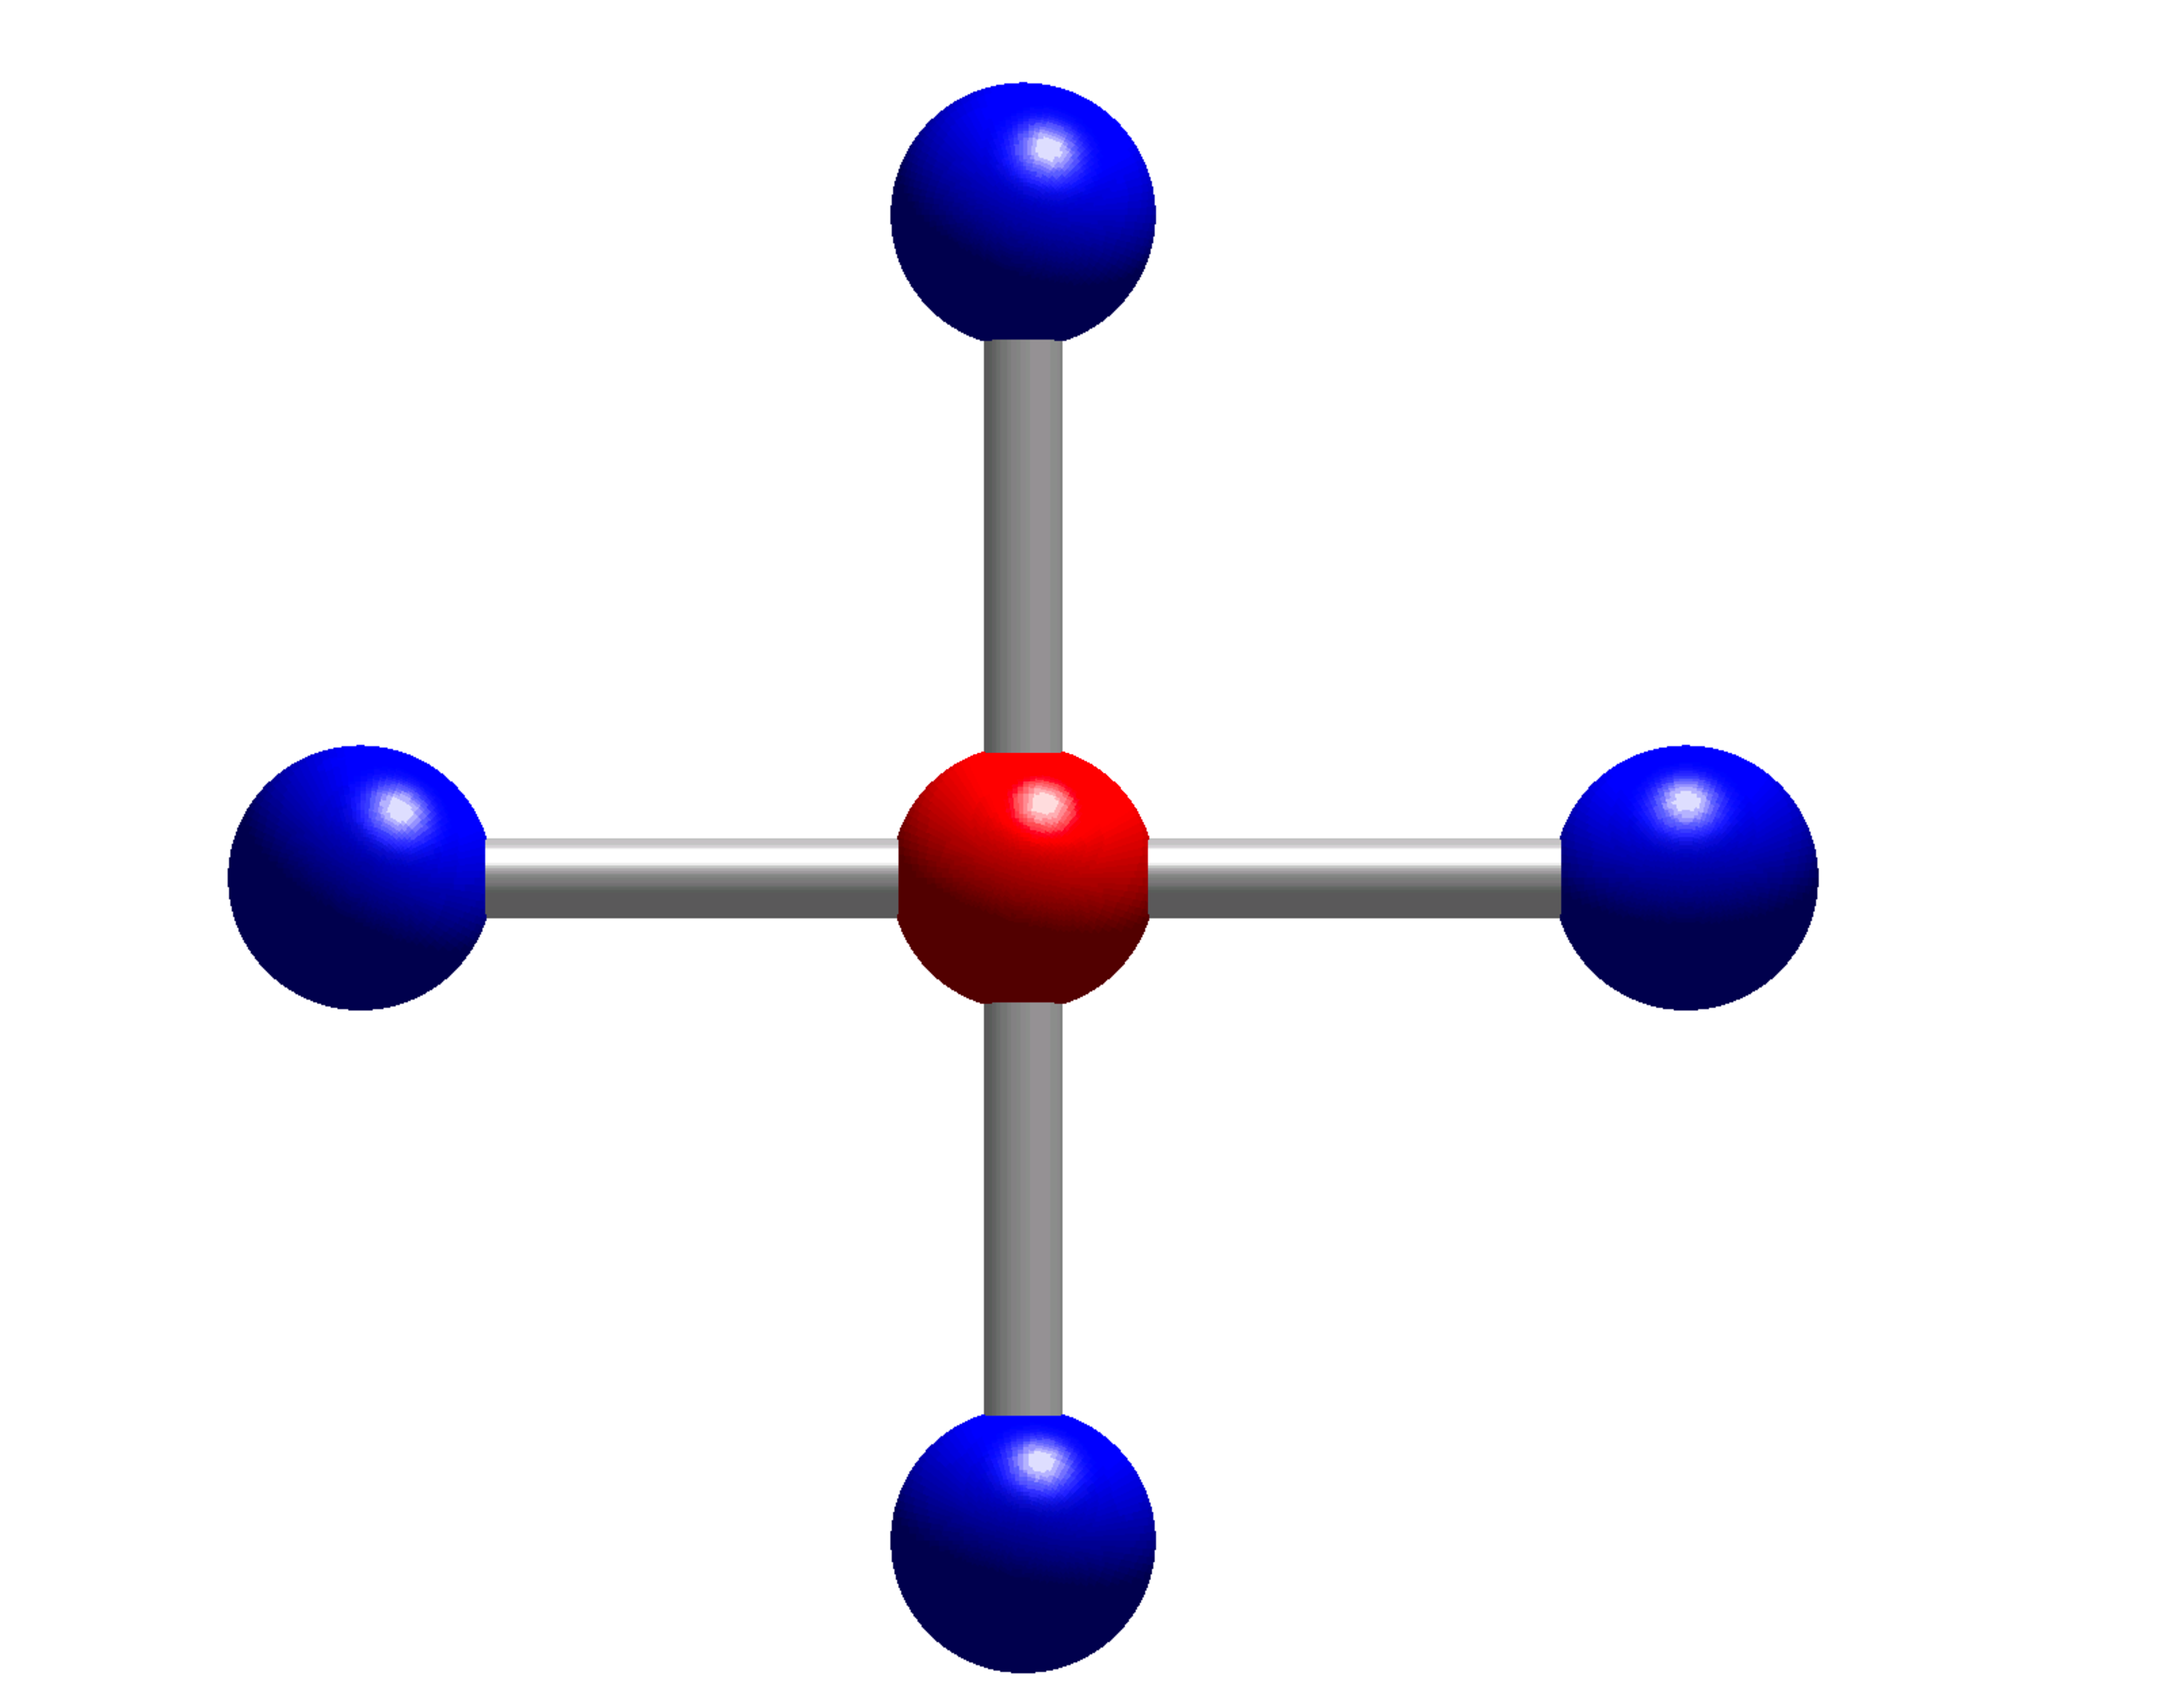
\includegraphics[width=\textwidth]{Stencil.pdf}

      2D Wilson stencil
      
      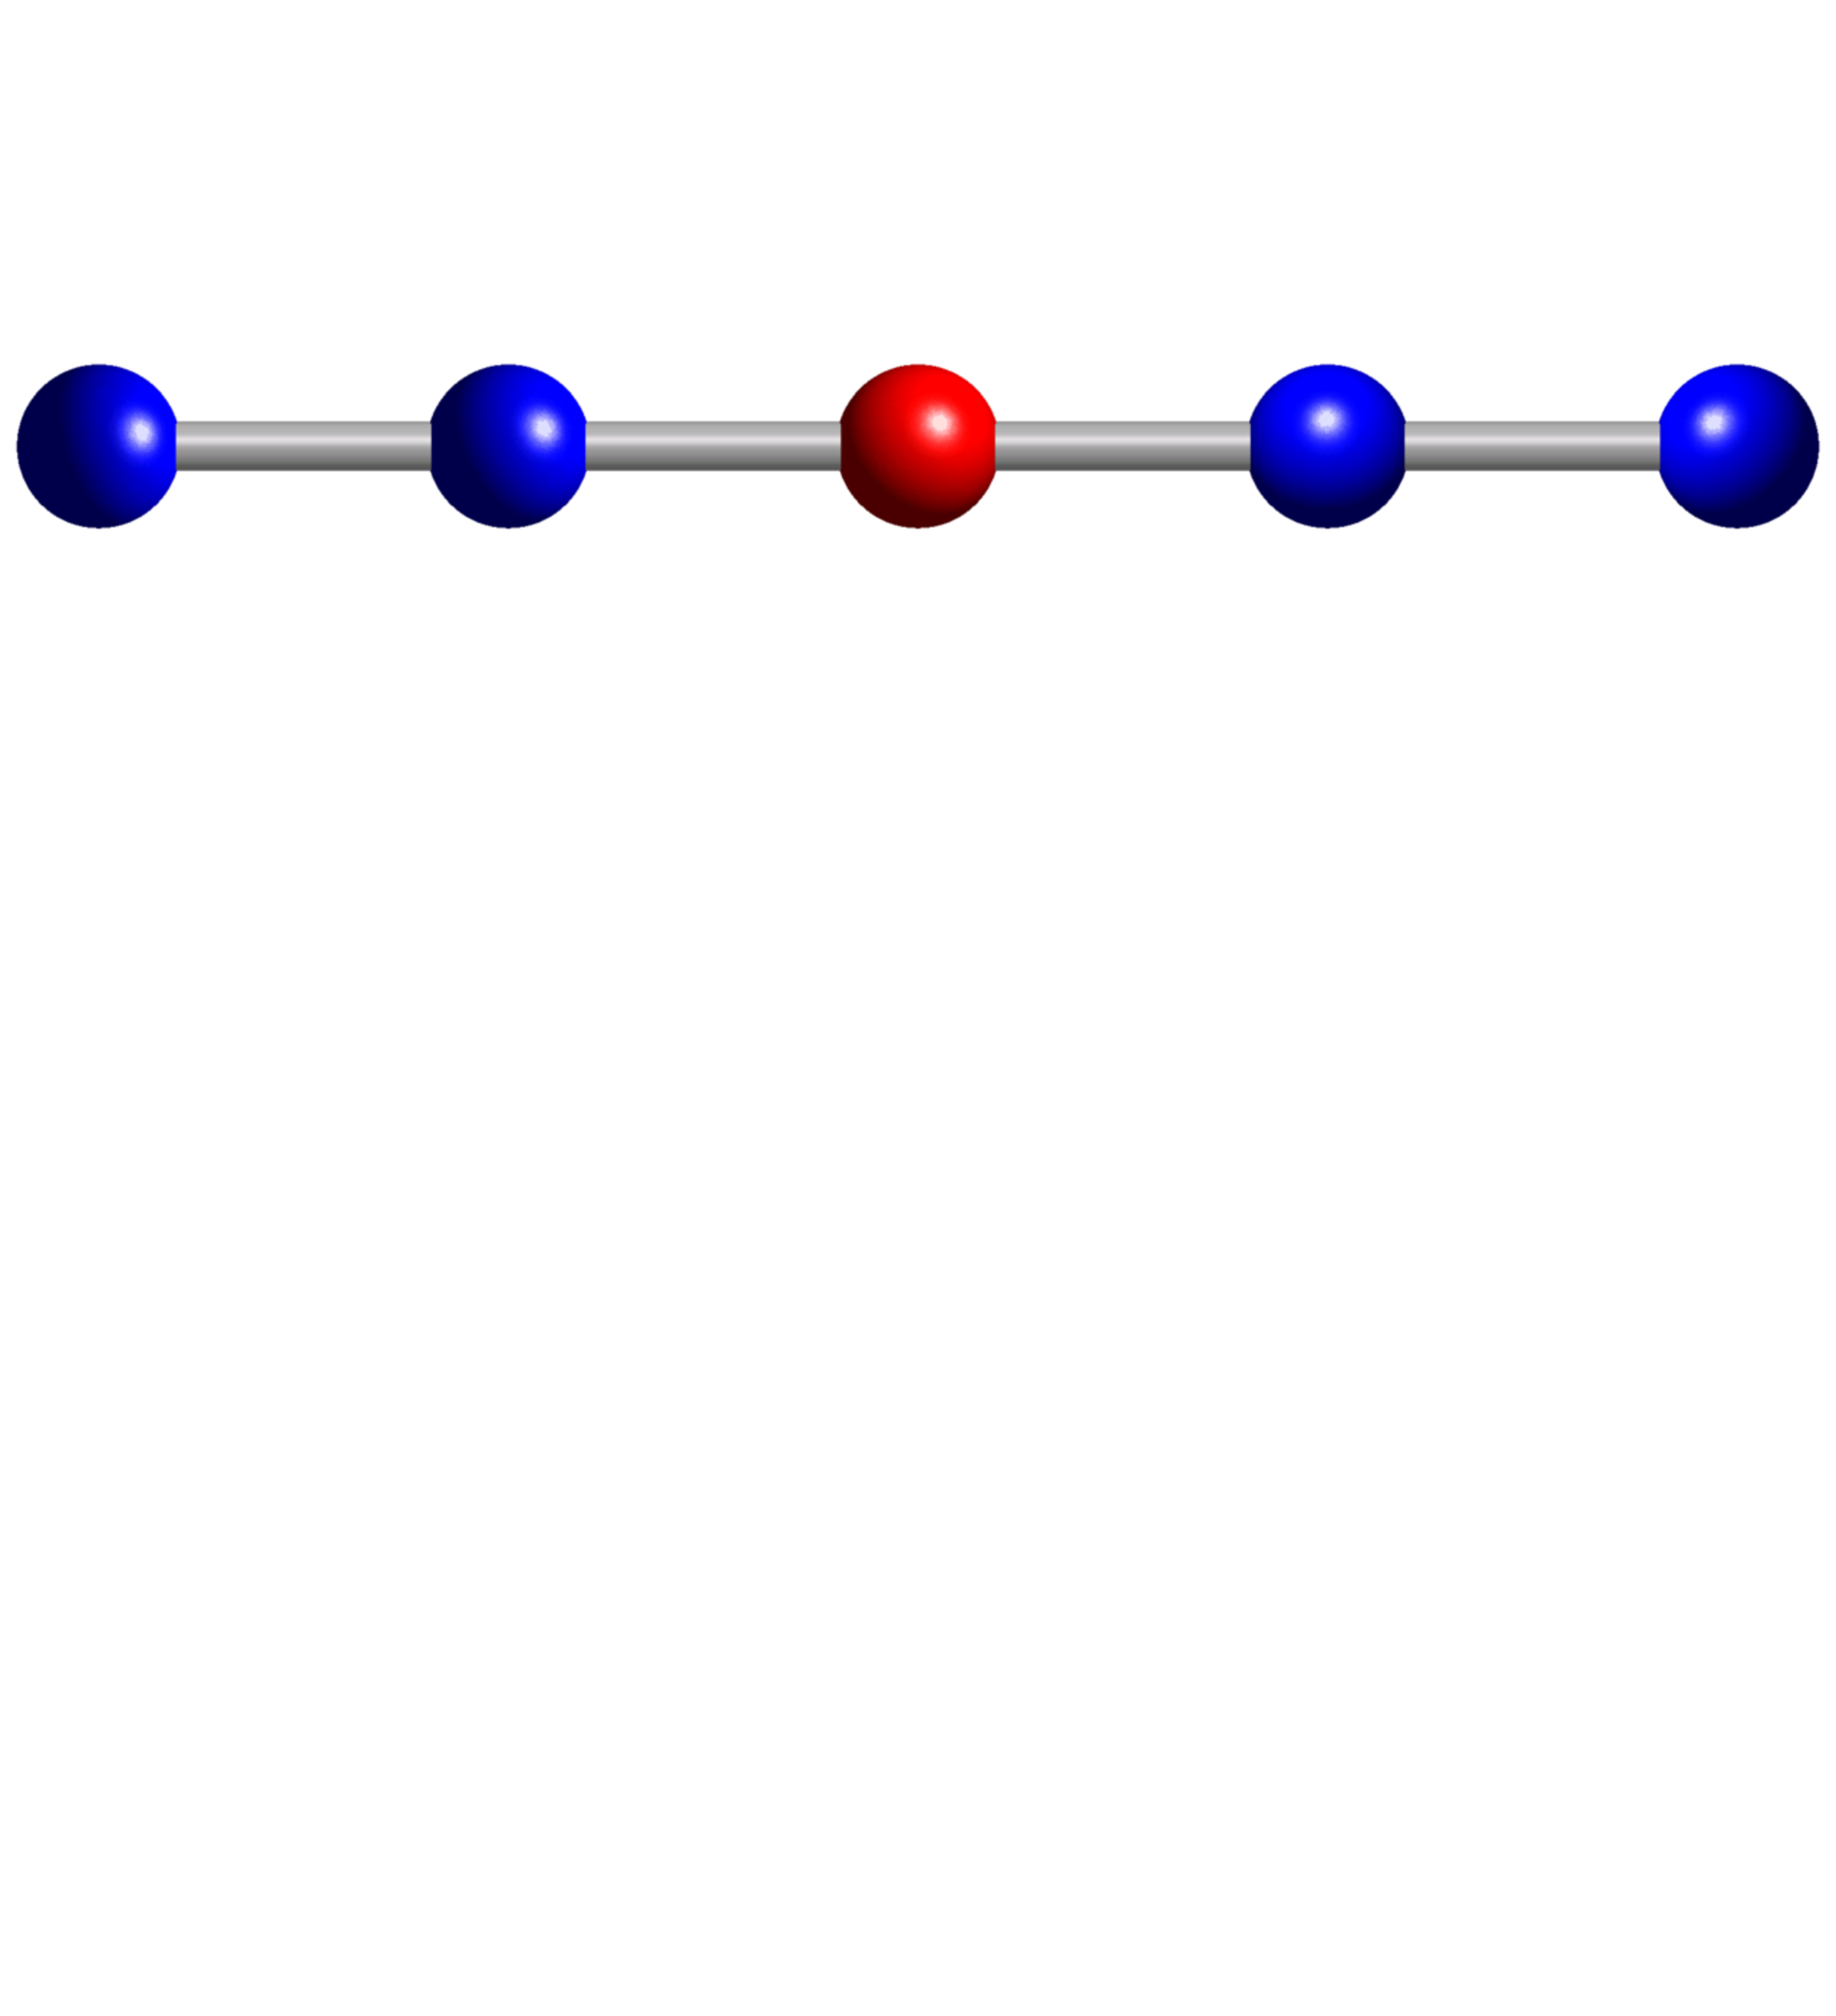
\includegraphics[width=\textwidth]{StencilNaik.pdf}

      Higher order derivative stencil

    \begin{eqnarray*}
      \begin{array}{c} c_1 (e^{ip_\mu} - e^{-ip_\mu}) \\ + c_2 (e^{i2 p_\mu} - e^{-i2 p_\mu})\end{array} \\
      \to  i p_\mu + O(p_\mu^5)
      \end{eqnarray*}
    \end{column}
  \end{columns}
\end{frame}

\begin{frame}[fragile]\small\frametitle{Stencils in Grid code}

\begin{itemize}
\item Grid provides a Stencil object, templated for any field
\begin{itemize}
\item Geometrical object only: decouples data motion (MPI, halo exchange), data access (indexing) from;
\item Algebra on internal indices (multiplying by gauge links, spinor structures, etc)
\end{itemize}
\item Compressor: object knows about Wilson spin projection (2spin/4spin), reduced precision
\item User writes a (node local) computational kernel that encodes the physics / internal index manipulation
\item Stencil object performs the data motion and presents neighbour tables
\end{itemize}

\end{frame}

\begin{frame}[fragile]\small\frametitle{ What is a CPU execution unit}

  \begin{itemize}
  \item One instruction fetch entity: fetches and decodes sequential instuctions until it hits a ``branch''
  \item One \emph{stack pointer} for function data
  \item (16) Scalar integer registers for address calculations (pointers, 8 bytes)
  \item (32) Vector floating point registers (e.g. 64 byte wide, or 16 single precision words)
  \item Vector loads contiguous data, naturally aligned
    \end{itemize}
  
\end{frame}

\begin{frame}[fragile]\small\frametitle{ What is a GPU execution unit}

\link{https://docs.nvidia.com/cuda/ampere-tuning-guide/index.html}
  
  \begin{itemize}
  \item Up to 64 instruction fetch entities (warps): fetches and decodes sequential instuctions until it hits a ``branch''
  \item Each instruction fetch controls up to 32 arithmetic units \& 32 columns of register file
  \item Vector integer registers (32 words) for address calculations (pointers)
  \item 32 \emph{stack pointers} for function data per warp\\
        these will be ``related'' to each other if all threads in warp make the same branches and calls
  \item Vector floating point registers (32 words)
  \item Vector loads can load unrelated data; contiguous data cases are dynamically detected and optimised in hardware\\
         Nvidia calls this ``coalesced  reads/writes''
    
    \end{itemize}

\end{frame}

\begin{frame}[fragile]\small\frametitle{ What is a GPU execution unit}

  \href{https://docs.nvidia.com/cuda/cuda-c-programming-guide/index.html#simt-architecture}
        {\color{blue}https://docs.nvidia.com/cuda/cuda-c-programming-guide/index.html\#simt-architecture}

  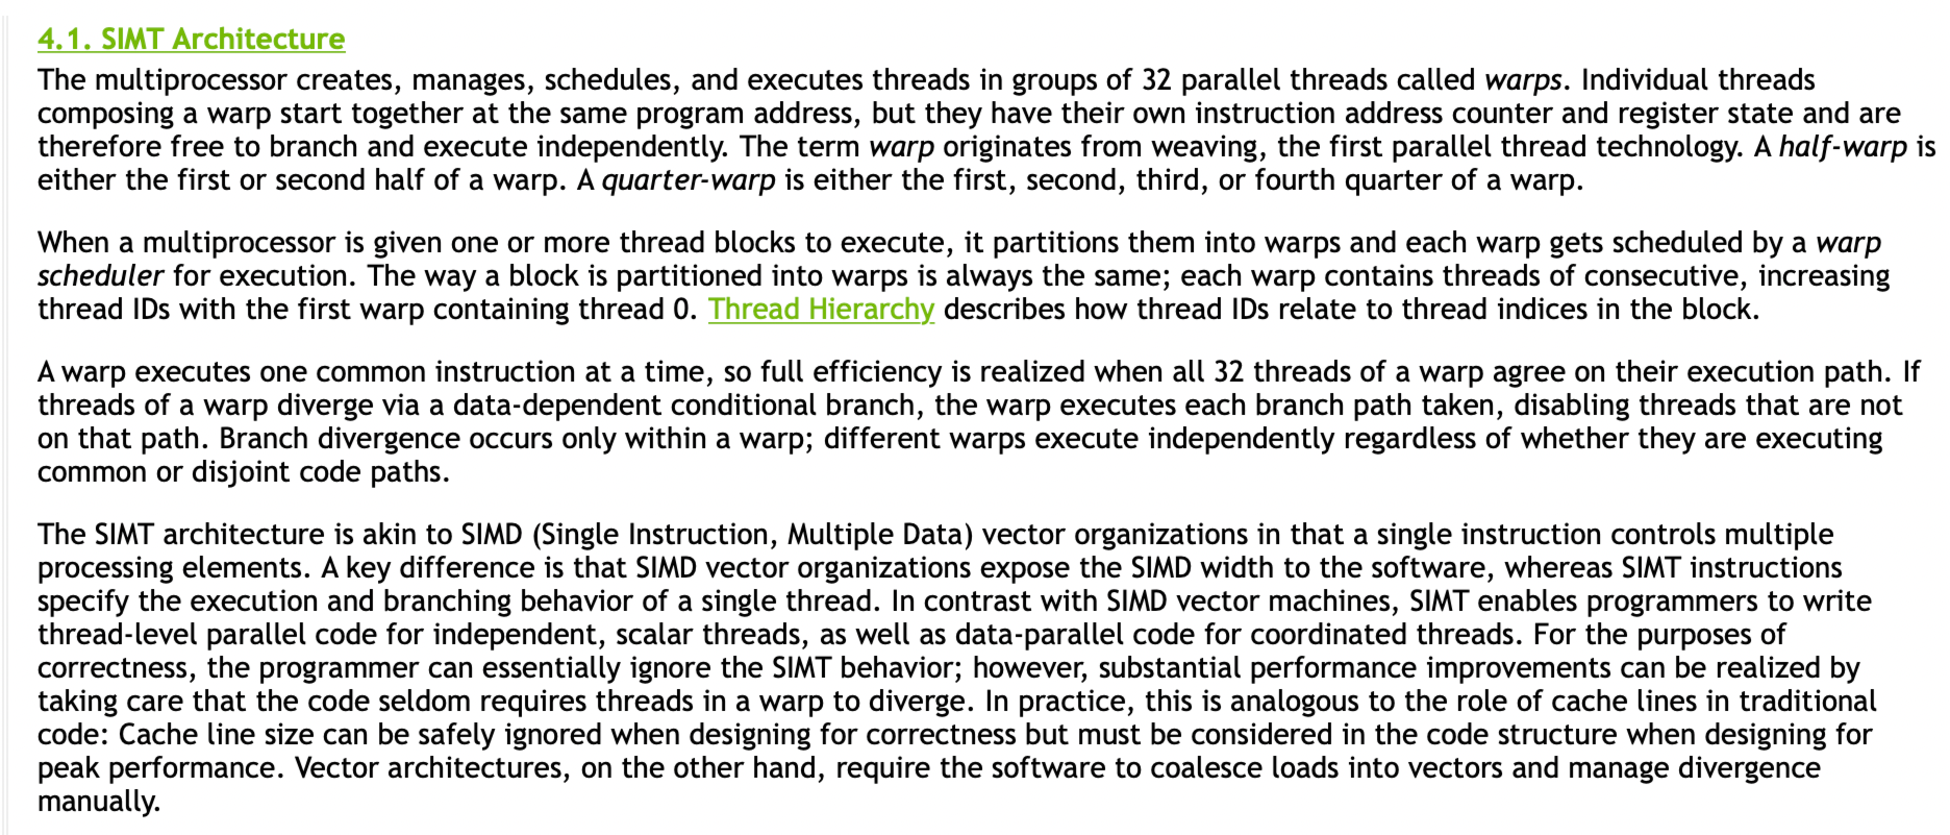
\includegraphics[width=\textwidth]{NvidiasWords.pdf}
  
\end{frame}

\begin{frame}[fragile]\small\frametitle{ How do you programme for both at a low level?}
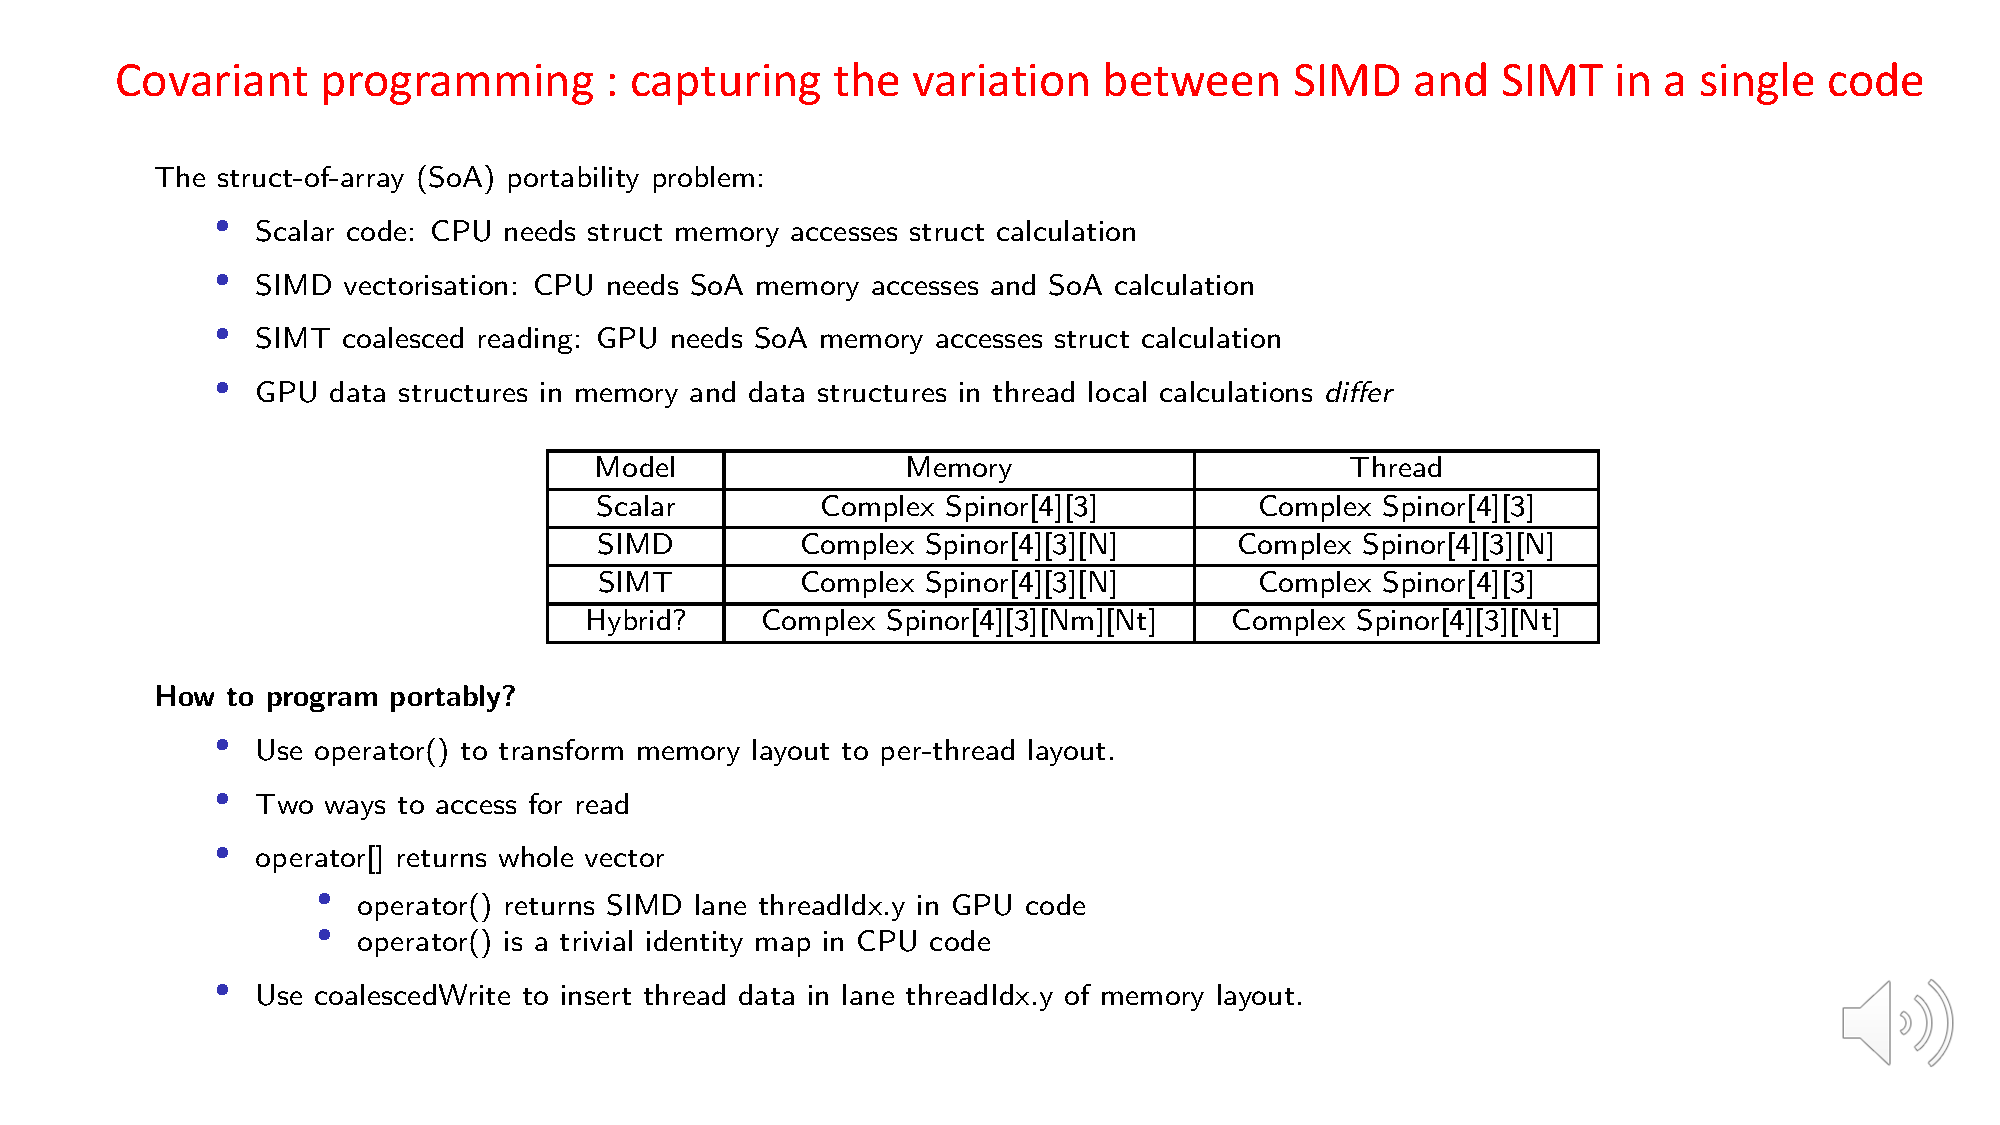
\includegraphics[width=\textwidth]{SIMD_SIMT.pdf}
\end{frame}
\begin{frame}[fragile]\small\frametitle{ How do you programme for both at a low level?}
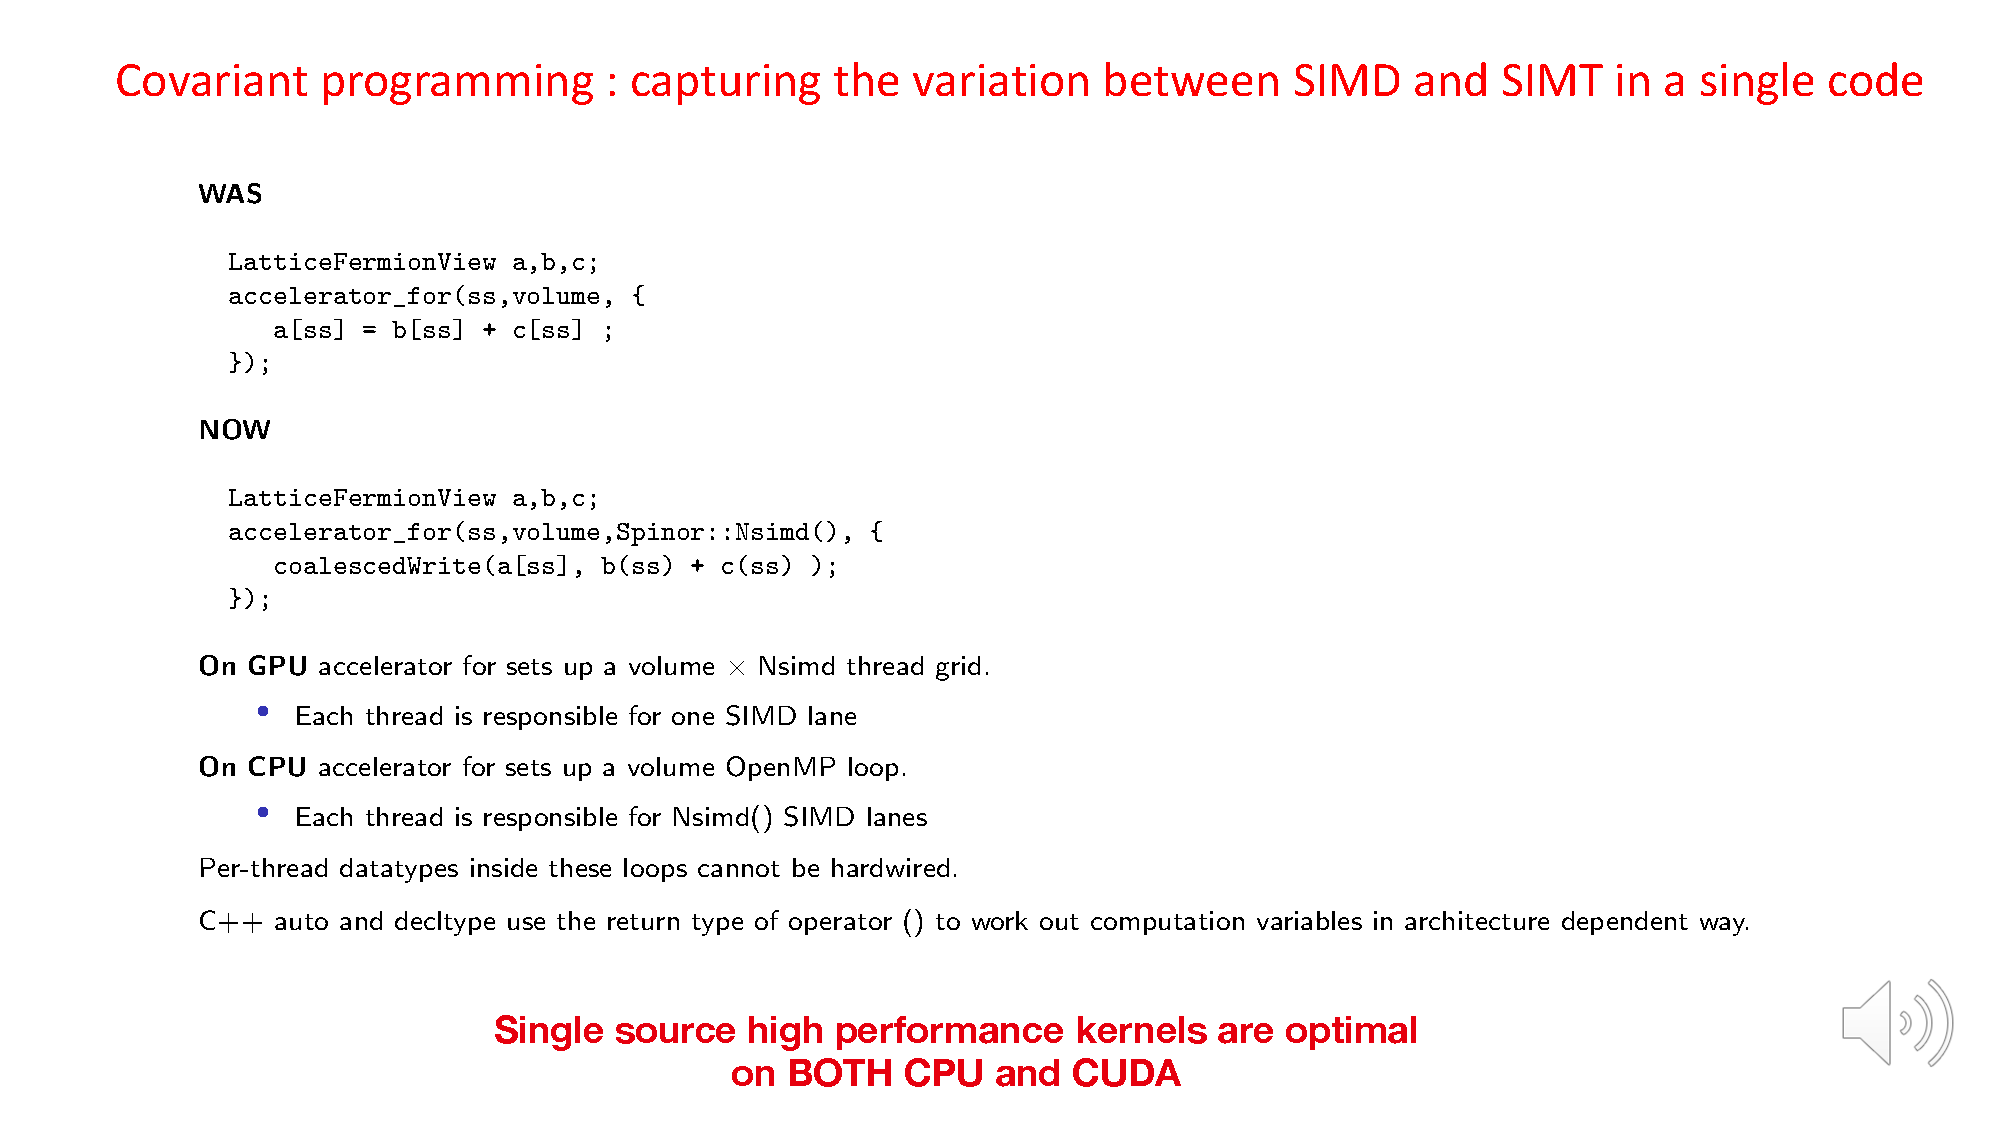
\includegraphics[width=\textwidth]{SIMD_SIMT_2.pdf}
\end{frame}

\begin{frame}[fragile]\small\frametitle{ How do you programme for multiple offload APIs?}
  \begin{itemize}
  \item Capture loop bodies in a (variadic) macro: abstract the interface to offload
  \begin{itemize}
    \item Here variadic = ``comma safe''
  \end{itemize}
  \link{https://github.com/paboyle/Grid/blob/develop/Grid/threads/Accelerator.h}
  \item Grid uses the \emph{accelerator\_for} and \emph{thread\_for} macros to 
  \item Think twice before using: \emph{most} code should be using data parallel expression templates
  \item Hadrons contains (almost?) \emph{no} cases of thread/accelerator for loops
  \item Interface is subject to change in future, so if you need it submit a function to Grid
  \end{itemize}
\end{frame}

\begin{frame}[fragile]\small\frametitle{ How do you ensure contiguous accesses?}
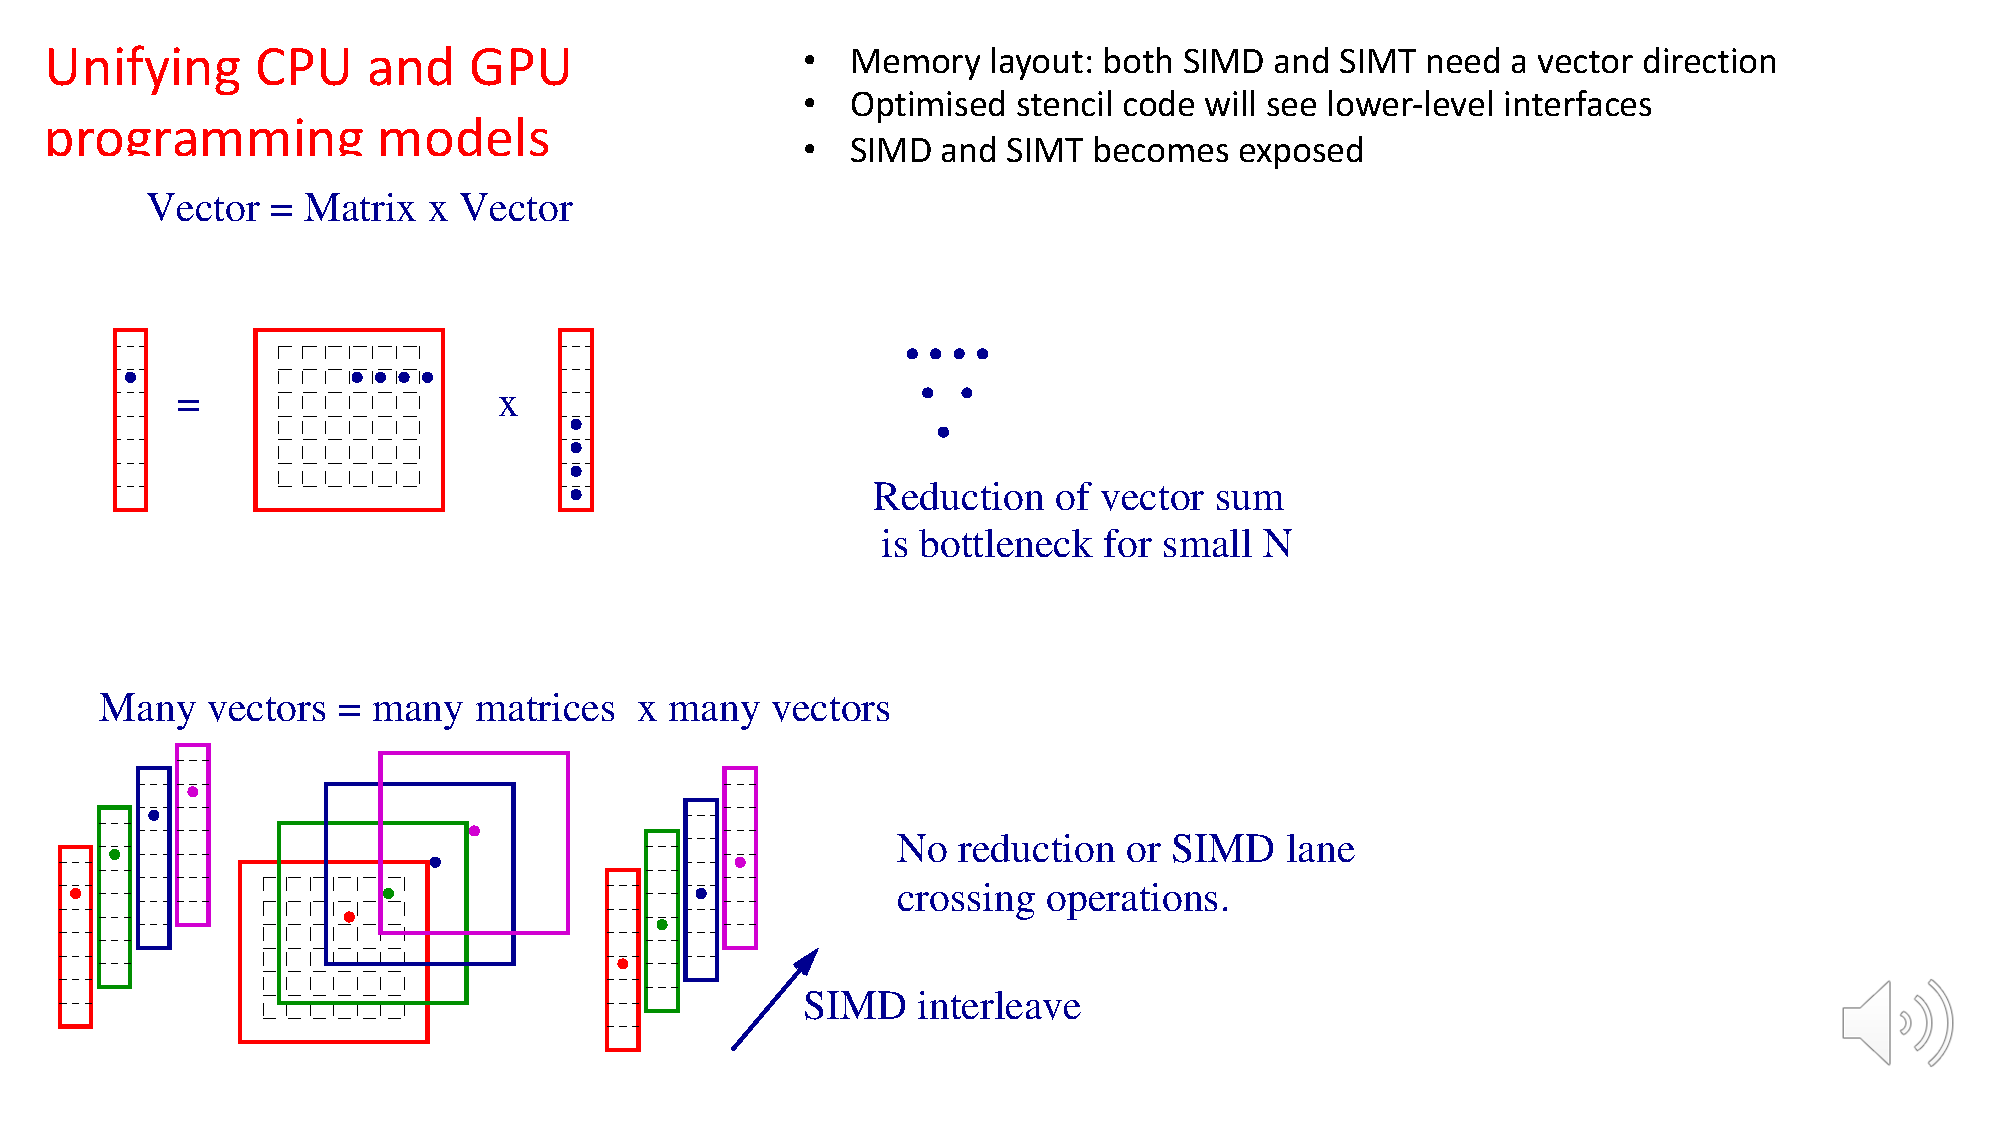
\includegraphics[width=0.8\textwidth]{Vectorise1.pdf}
\end{frame}
\begin{frame}[fragile]\small\frametitle{ How do you ensure contiguous accesses?}
  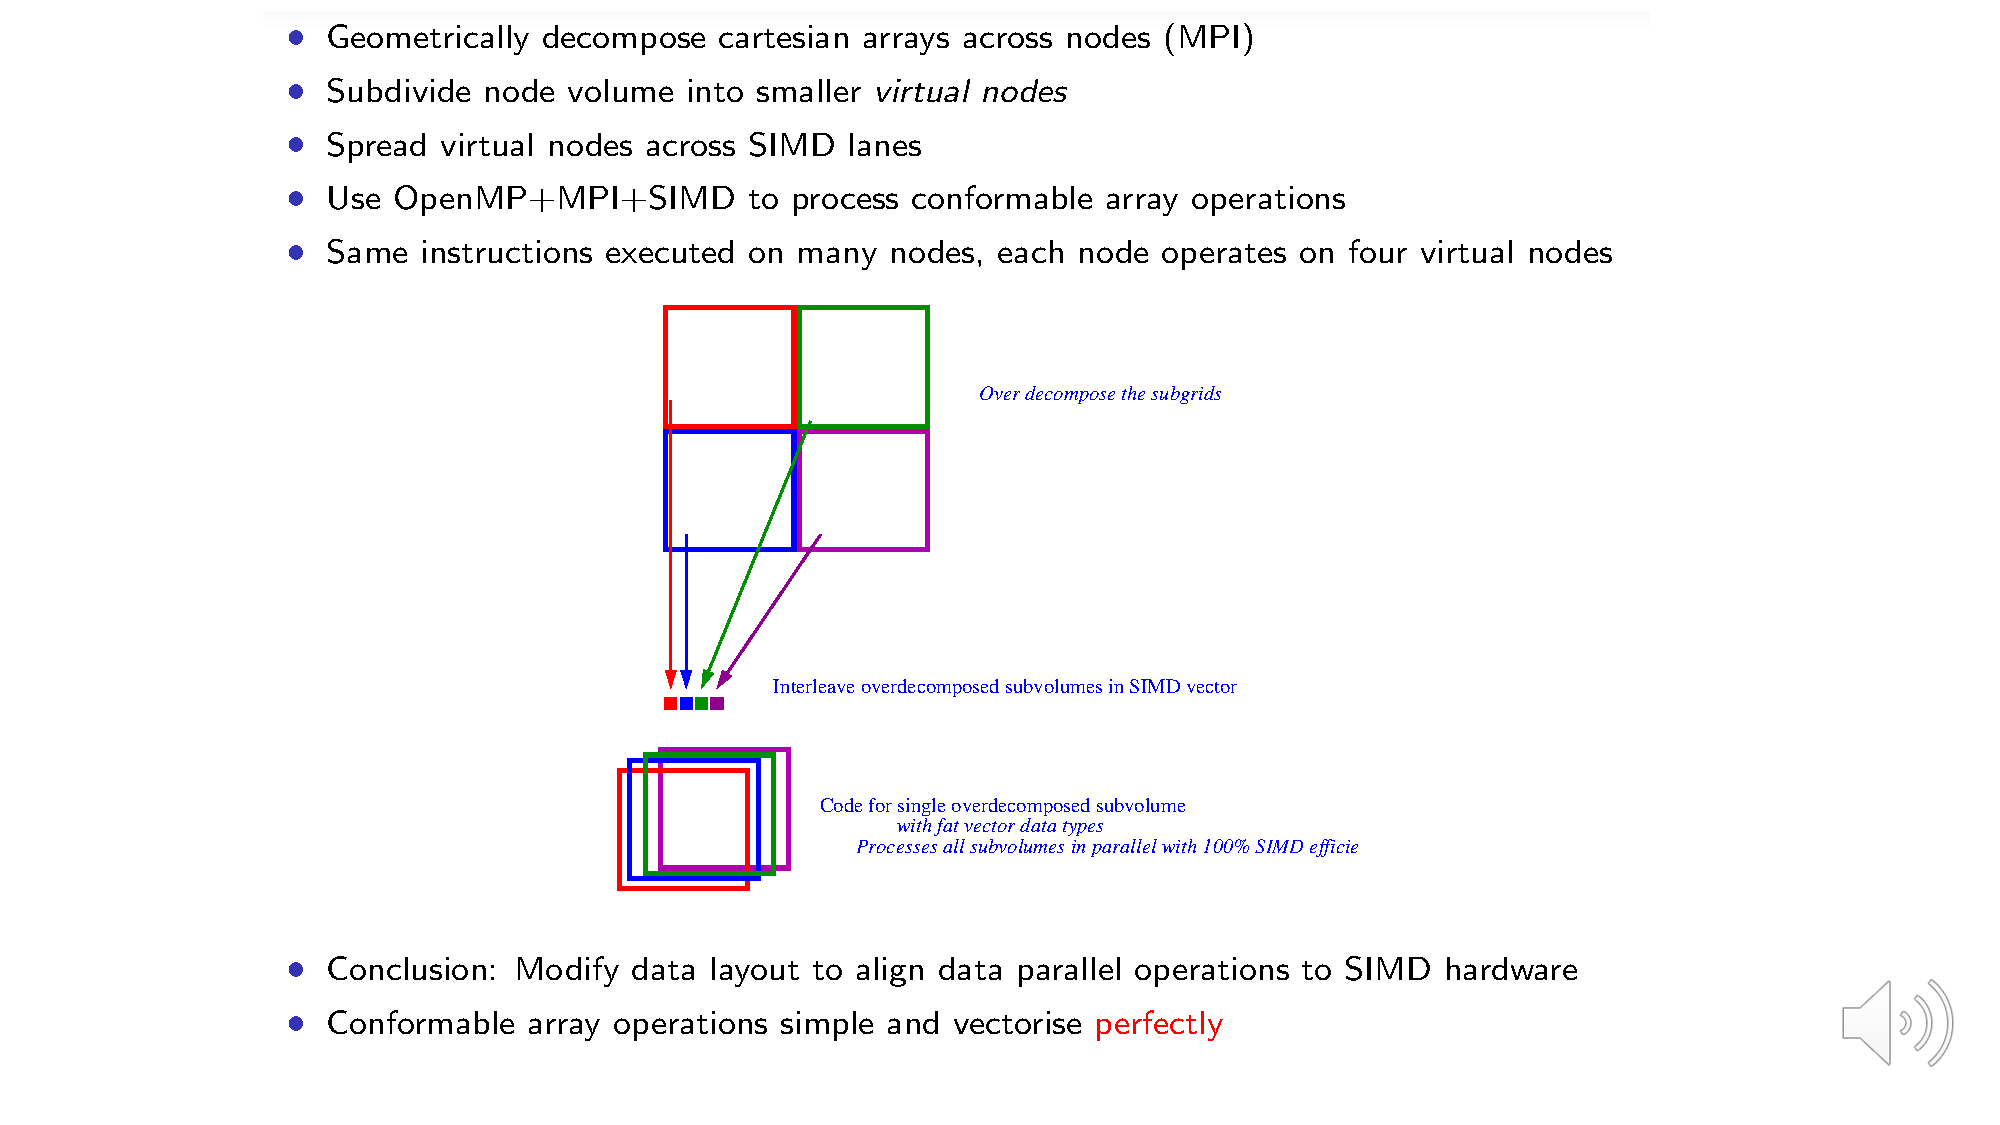
\includegraphics[width=0.8\textwidth]{Vectorise2.pdf}
  \begin{center}
    {\tiny Must permute red/green/blue/purple when you access off the edge of sub-cell }
\end{center}  
\end{frame}

\begin{frame}[fragile]\small\frametitle{ How can you manage memory?}
  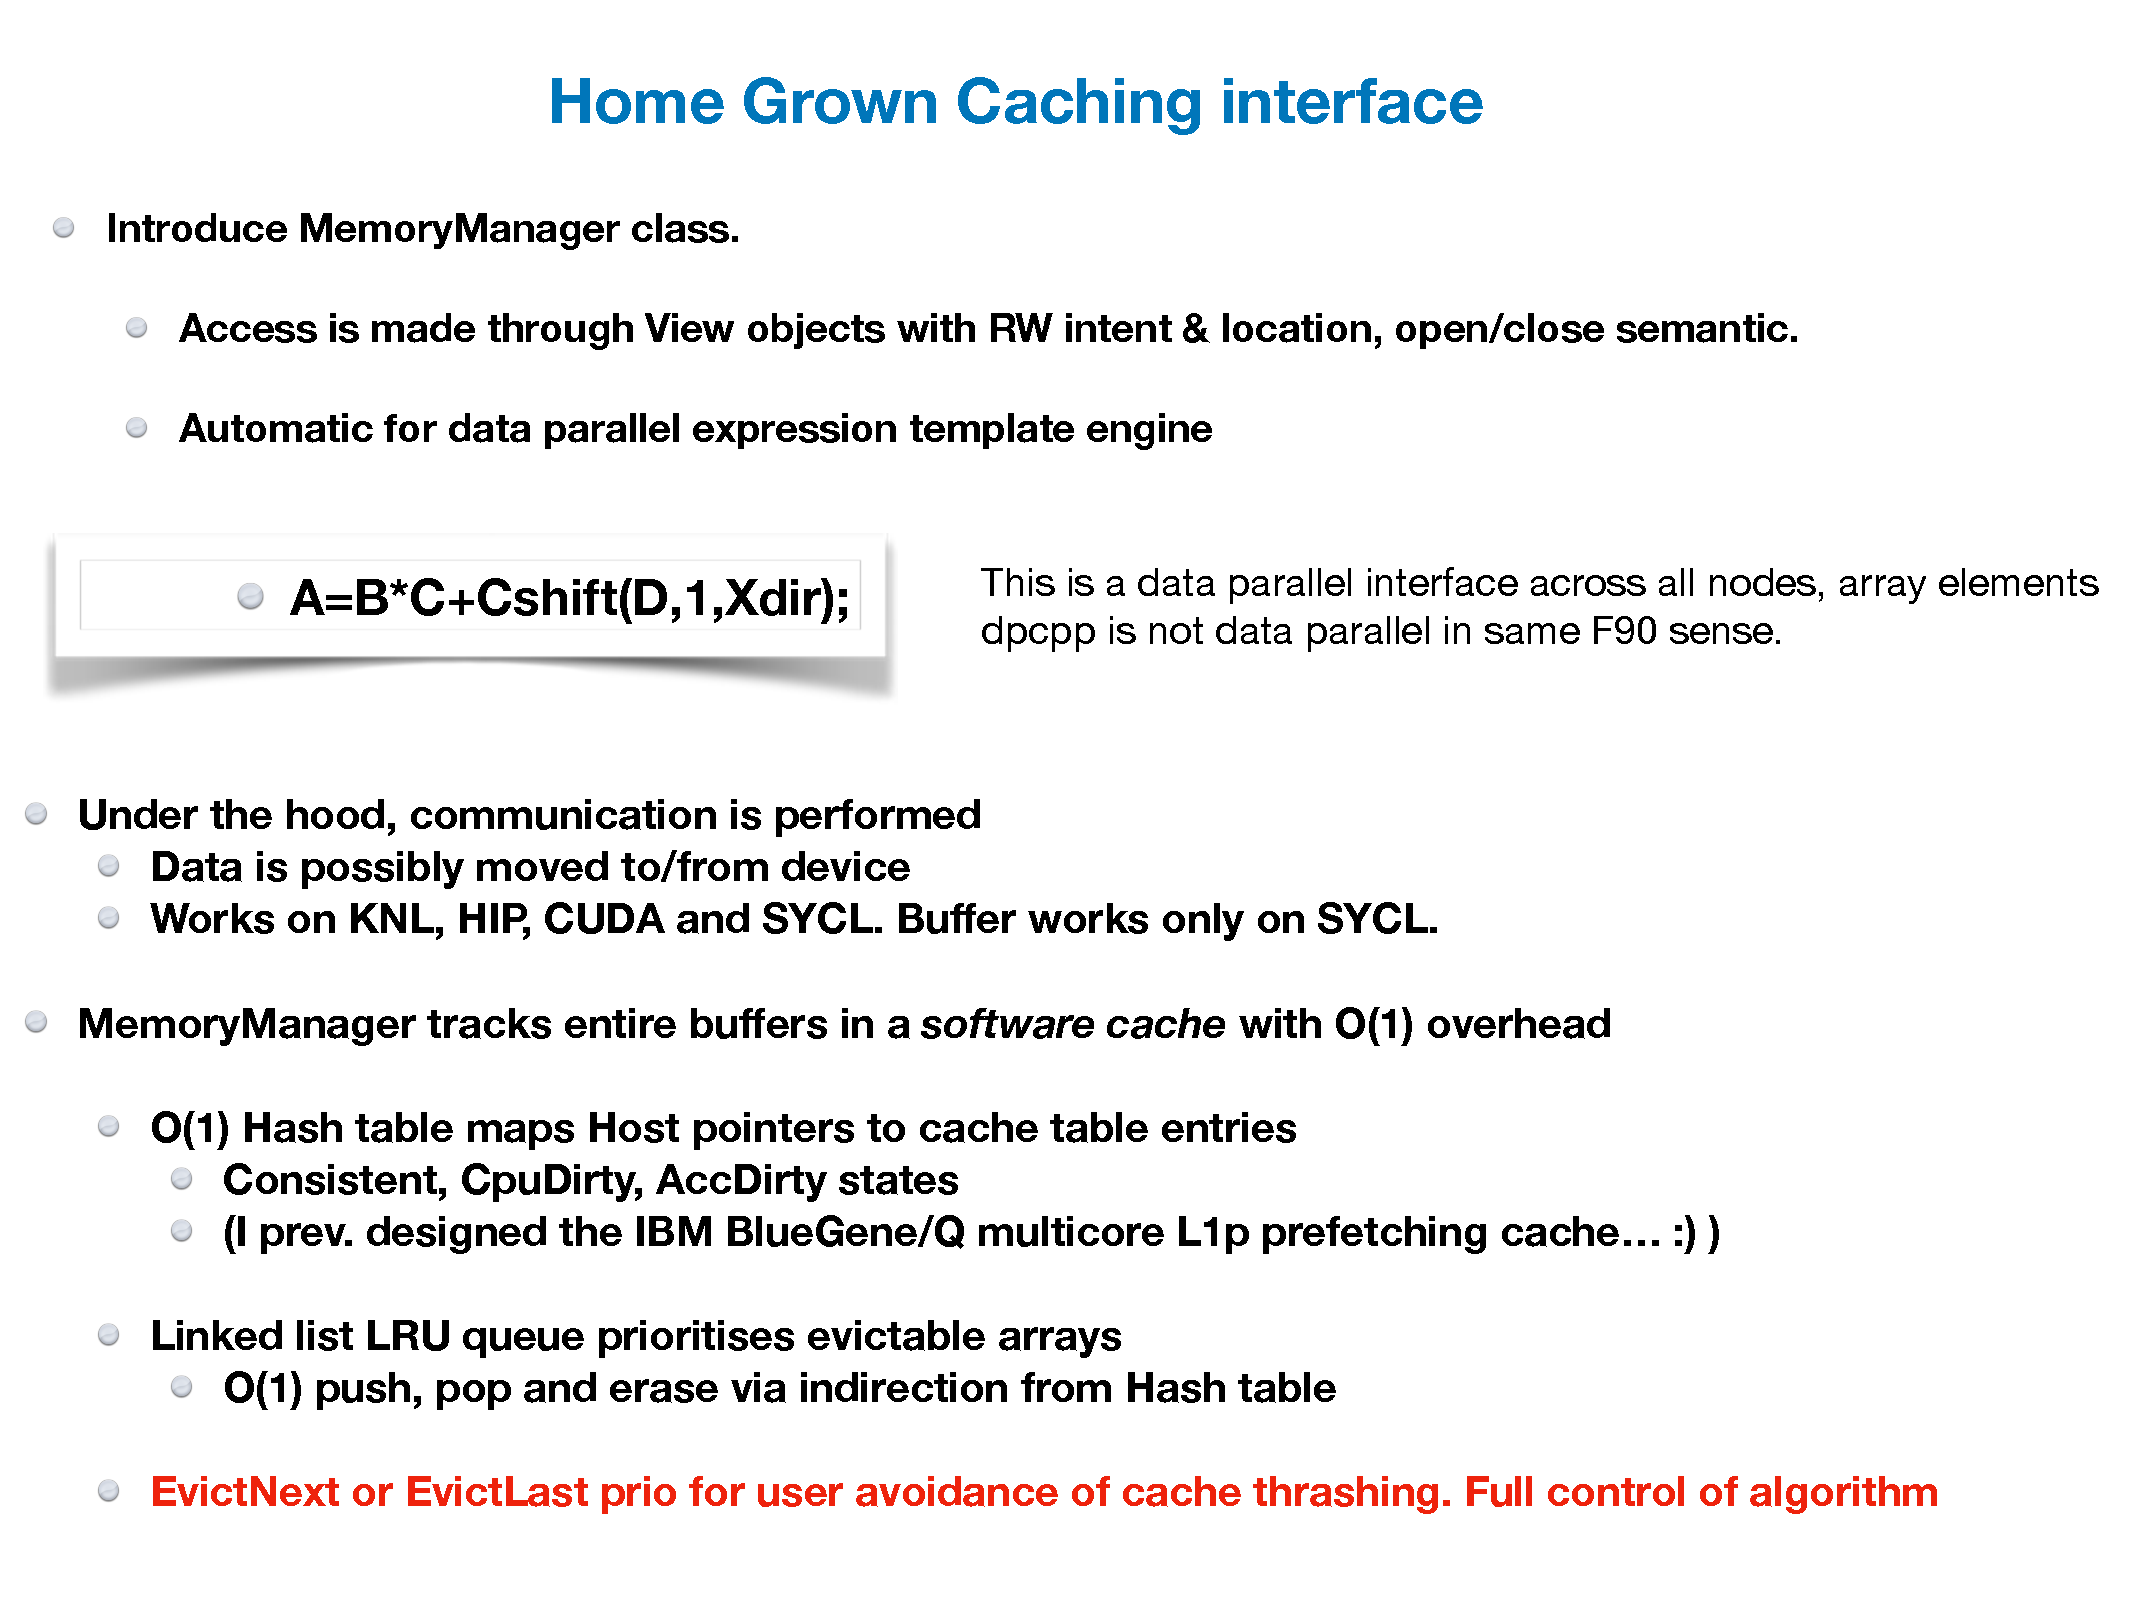
\includegraphics[width=0.8\textwidth]{Caching.pdf}

  \begin{center}
    \begin{itemize}
    \begin{itemize}
    \item Must obtain a \emph{view} of an object for host/acccelerator from software cache manager - returns pointer to use
    \item Memory manager triggers data motion if required
    \item Configure option: --enable-unified=yes/no
    \end{itemize}
    \end{itemize}
  \end{center}
\end{frame}

\begin{frame}[fragile]\small\frametitle{ Stencil implementation of free Laplacian}
{\miniscule
\begin{verbatim}
template<class Field> class FreeLaplacianStencil : public SparseMatrixBase<Field>
{
  typedef typename Field::vector_object siteObject;
  typedef CartesianStencil<siteObject, siteObject, int> StencilImpl;

  StencilImpl Stencil;
  SimpleCompressor<siteObject> Compressor;

  FreeLaplacianStencil(GridBase *_grid) : Stencil    (_grid,6,Even,directions,displacements,0), grid(_grid) {};

  virtual void  M    (const Field &_in, Field &_out)
  {
    Stencil.HaloExchange(_in, Compressor);     // Halo exchange for this geometry of stencil

    auto buf = st.CommBuf();
    auto st = Stencil.View(AcceleratorRead);       // Views; device friendly/accessible pointers
    autoView( in     , _in    , AcceleratorRead);
    autoView( out    , _out   , AcceleratorWrite);

    typedef typename Field::vector_object     vobj;
    typedef decltype(coalescedRead(in[0])) calcObj;
    const int      Nsimd = vobj::Nsimd();
    const uint64_t NN = grid->oSites();

    accelerator_for( ss, NN, Nsimd, {

        StencilEntry *SE;
        const int lane=acceleratorSIMTlane(Nsimd);
        calcObj chi, res;

#define LEG_LOAD(Dir)                                            \
  SE = st.GetEntry(ptype, Dir, ss);                              \
  if (SE->_is_local ) {                                          \
    int perm= SE->_permute;                                      \
    chi = coalescedReadPermute(in[SE->_offset],ptype,perm,lane); \
  } else {                                                       \
    chi = coalescedRead(buf[SE->_offset],lane);                  \
  }                                                              \
  acceleratorSynchronise();

        res                 = coalescedRead(in[ss])*(-6.0);
        LEG_LOAD(0);	res = res + chi;
        LEG_LOAD(1);	res = res + chi;
        LEG_LOAD(2);	res = res + chi;
        LEG_LOAD(3);	res = res + chi;
        LEG_LOAD(4);	res = res + chi;
        LEG_LOAD(5);	res = res + chi;

        coalescedWrite(out[ss], res,lane);
    });
  };
};
\end{verbatim}
}
\end{frame}

\begin{frame}[fragile]\small\frametitle{ Stencil implementation of covariant Laplacian}
{\miniscule
\begin{verbatim}
template<class Gimpl,class Field> class CovariantLaplacianStencil : public SparseMatrixBase<Field>
{
  StencilImpl Stencil;
  SimpleCompressor<siteObject> Compressor;
  DoubledGaugeField Uds;

  CovariantLaplacianStencil(GaugeField &Umu) : grid(Umu.Grid()), Stencil(grid,6,Even,directions,displacements,0), Uds(grid)
  {
    for (int mu = 0; mu < Nd; mu++) {
      auto U = PeekIndex<LorentzIndex>(Umu, mu);
      PokeIndex<LorentzIndex>(Uds, U, mu );
      U = adj(Cshift(U, mu, -1));   // Double store gauge field (8 links per site)
      PokeIndex<LorentzIndex>(Uds, U, mu + 4);
    }
  };

  virtual void  M    (const Field &_in, Field &_out)
  {
    Stencil.HaloExchange(_in, Compressor);// Halo exchange for this geometry of stencil

    // Arithmetic expressions
    auto st = Stencil.View(AcceleratorRead);
    auto buf = st.CommBuf();

    autoView( in     , _in    , AcceleratorRead);
    autoView( out    , _out   , AcceleratorWrite);
    autoView( U     , Uds    , AcceleratorRead);

    typedef typename Field::vector_object        vobj;
    typedef decltype(coalescedRead(in[0]))    calcObj;
    typedef decltype(coalescedRead(U[0](0))) calcLink;

    const int      Nsimd = vobj::Nsimd();
    const uint64_t NN = grid->oSites();
    accelerator_for( ss, NN, Nsimd, {

        StencilEntry *SE;
        const int lane=acceleratorSIMTlane(Nsimd);
        calcObj chi, res;
        calcLink UU;

#define LEG_LOAD_MULT(leg,polarisation)	\
        UU = coalescedRead(U[ss](polarisation)); \
        LEG_LOAD(leg); \
        res = res + UU*chi();			        
	
        res                 = coalescedRead(in[ss])*(-6.0);
        LEG_LOAD_MULT(0,Xp);
        LEG_LOAD_MULT(1,Yp);
        LEG_LOAD_MULT(2,Zp);
        LEG_LOAD_MULT(3,Xm);
        LEG_LOAD_MULT(4,Ym);
        LEG_LOAD_MULT(5,Zm);

        coalescedWrite(out[ss], res,lane);
    });
  };
};
\end{verbatim}
}
\end{frame}



\begin{frame}[fragile]\small\frametitle{Scalar propagator}

  \begin{itemize}
  \item $S = \phi^\ast (\Box  + m^2) \phi $
    $$
      M(x,x^\prime) = \delta_{x,x^\prime} 2( N_d+m^2 ) - \sum\limits_\mu \delta_{x+\mu,x^\prime}+\delta_{x-\mu,x^\prime}
        $$
      \item {\bf Free case:} M is hermitian diagonalised by a unitary transformation
        $$
        M = V^\dagger D V
        $$
      \item Call it the ``discrete fourier transform'' in the free case, and the eigenvalues are
        $$
        D(p) = (2 \sin p/2)^2 + m^2
        $$
  \begin{itemize}
      \item Propagator is the inverse of this
  \end{itemize}
      \item {\bf Interacting case:} M is hermitian diagonalised by a unitary transformation
        $$
        M = V^\dagger D V
        $$
      \item covariant derivative couples to gauge fields, numerical solution of propagator
      \item Still diagonalisable, eigenvectors no longer plane waves etc...
$$M^{-1} = V \mathrm{Diag}\{ \frac{1}{\lambda_i} \} V^\dag \simeq  V \mathrm{Diag}\{ P(\lambda_i) \} V^\dag  $$
      \item If P is polynomial approximating $\frac{1}{x}$ over the whole spectral range $\Rightarrow$ Krylov solvers
  \end{itemize}
 \end{frame}

  \begin{frame}[fragile]\small\frametitle{ Covariant smearing}

    \begin{itemize}
    \item Base on free field Gaussian function:
      $$S(x) = \frac{1}{\sqrt{2\pi}\sigma} e^{-x^2/ 2\sigma^2} \Leftrightarrow \tilde S(p) = \frac{1}{\sqrt{2\pi}} e^{-p^2 \sigma^2/2}$$
    \item Approximate with fixed a polynomial:
    \begin{itemize}
       \item $e^{-x} \sim (1-\frac{x}{N})^N = \sum_n (N| n) (\frac{x^n}{N^n}) = \sum_n \frac{N!}{ N^n (N-n)!}  \frac{1}{n!} x^n \to \sum_n \frac{x_n}{n!}$
    \end{itemize}
    \item Where the limit is true term by term in the series; convergence will occur for fixed $x$ with large $N$
    \item Wuppertal smearing: apply this polynomial of covariant Laplacian $$\mathbb{P}(L) (x,y) \sim e^{|x-y|^2/2\sigma^2}$$
      \begin{itemize}
    \item It will convolve an input vector $b(y)$ with the Gaussian in the free field case
    \item Interacting case is the gauge covariant generalisation
     \end{itemize}
    \item Uses:
      \begin{itemize}
      \item $b(y) = \delta_{y,y_0}$  : Gaussian source at $y_0$
    \item $b(y) = \delta_{y_t,t_0} \mathbb{Z}_2(y)$  : (stochastic) Wall of Gaussian sources
    \item Sink smearing of a propagator
    \item Sequential sources for 3point functions, semileptonic form factors 
    \end{itemize}
    \end{itemize}
  \end{frame}

  \begin{frame}[fragile]\small\frametitle{ Covariant smearing}
Example implementation: \link{https://github.com/paboyle/Grid/blob/develop/Grid/qcd/utils/CovariantSmearing.h}
\begin{verbatim}
    // Free field iterates 
    //   chi = (1 - w^2/4N p^2)^N chi
    Real coeff = (width*width) / Real(4*Iterations);
  
    for(int n = 0; n < Iterations; ++n) {
      Laplacian.M(chi,psi);
      chi = chi + coeff*psi;
    }
\end{verbatim}

  \end{frame}

  \begin{frame}[fragile]\small\frametitle{ Chebyshev polynomials \& approximation}

    \begin{center}
    \link{https://github.com/paboyle/Grid/blob/develop/Grid/algorithms/approx/Chebyshev.h}
    \end{center}

    \begin{itemize}
    \item Chebyshev polynomials provide a general scheme for polynomial approximation over a given range
    \item Exponentially accurate in polynomial order
    \item Numerical Recipes in ``C'', chapter 5-8.
    \item Rational approximation chapter 5-13
\begin{center}    \link{http://numerical.recipes/book/book.html}\end{center}
    \item Can apply to any Hermitian matrix (not just function of one variable!)
    \item Disadvantage: must know upper and lower spectral bounds - not a \emph{black box method}
    \end{itemize}

         {\tiny
\begin{verbatim}
  void operator() (LinearOperatorBase<Field> &Linop, const Field &in, Field &out) 
\end{verbatim}
}

  \end{frame}

  \begin{frame}[fragile]\small\frametitle{ Chebyshev polynomials \& approximation}
\tiny
    \begin{columns}
      \begin{column}{0.5\textwidth}
        Orthogonal univariate polynomials on $[-1,1]$\\
        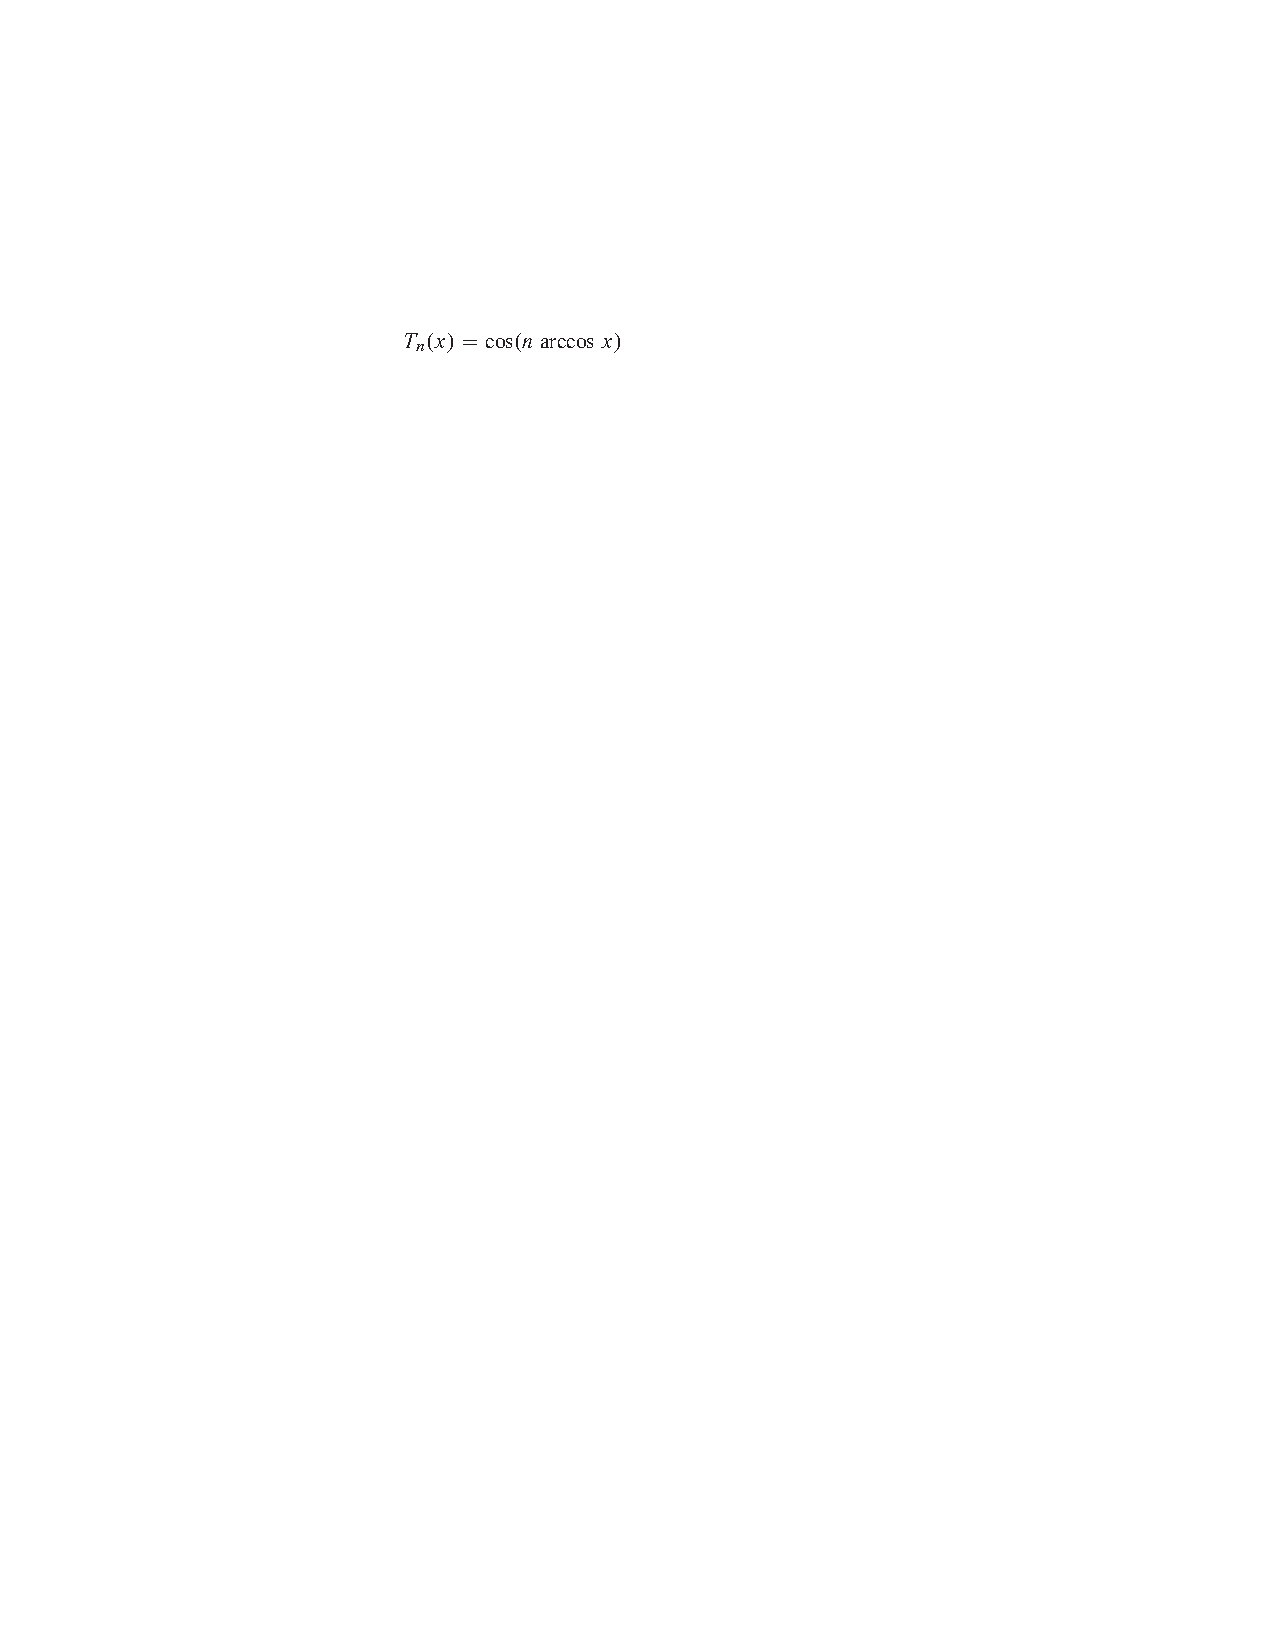
\includegraphics[width=0.5\textwidth]{ChebyCos.pdf}\\
        Recursion relation:\\
        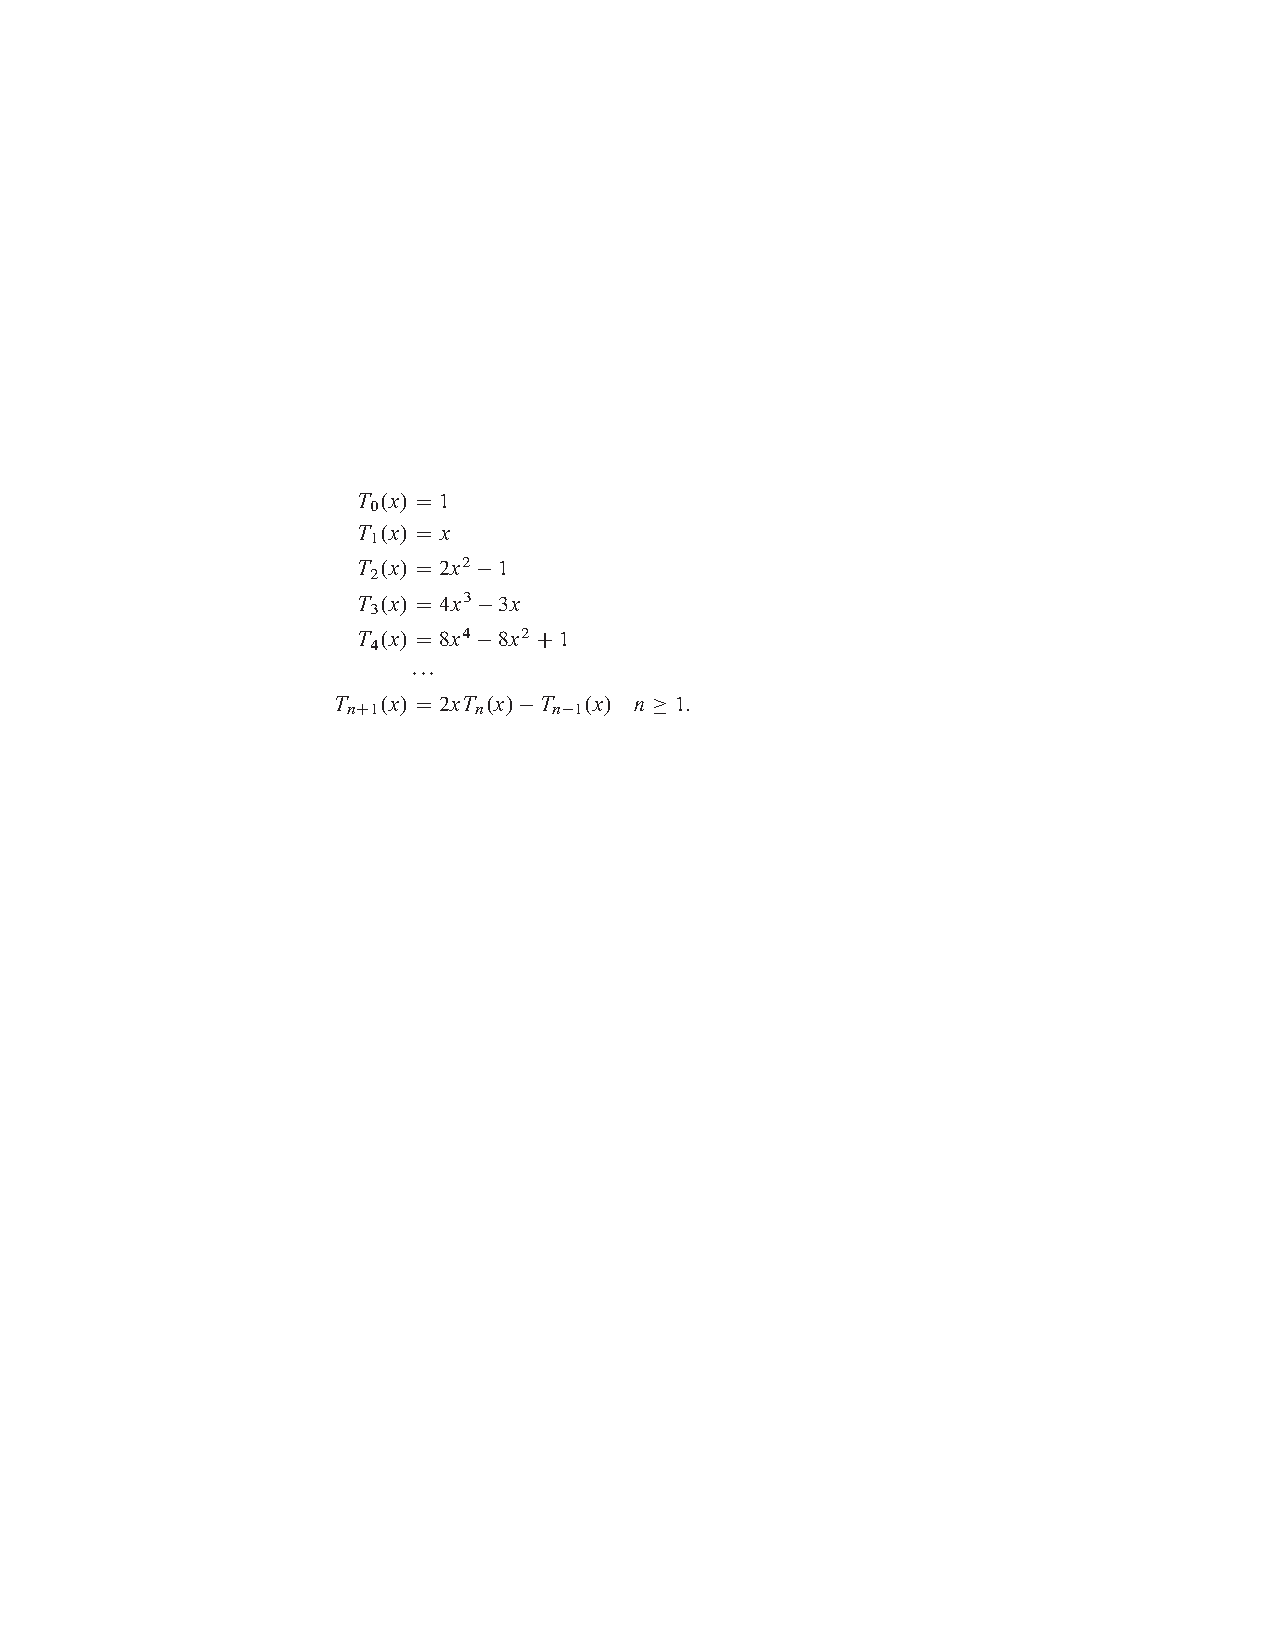
\includegraphics[width=0.8\textwidth]{ChebyRecursion.pdf}\\
        Chebyshev expansion coefficients:\\
        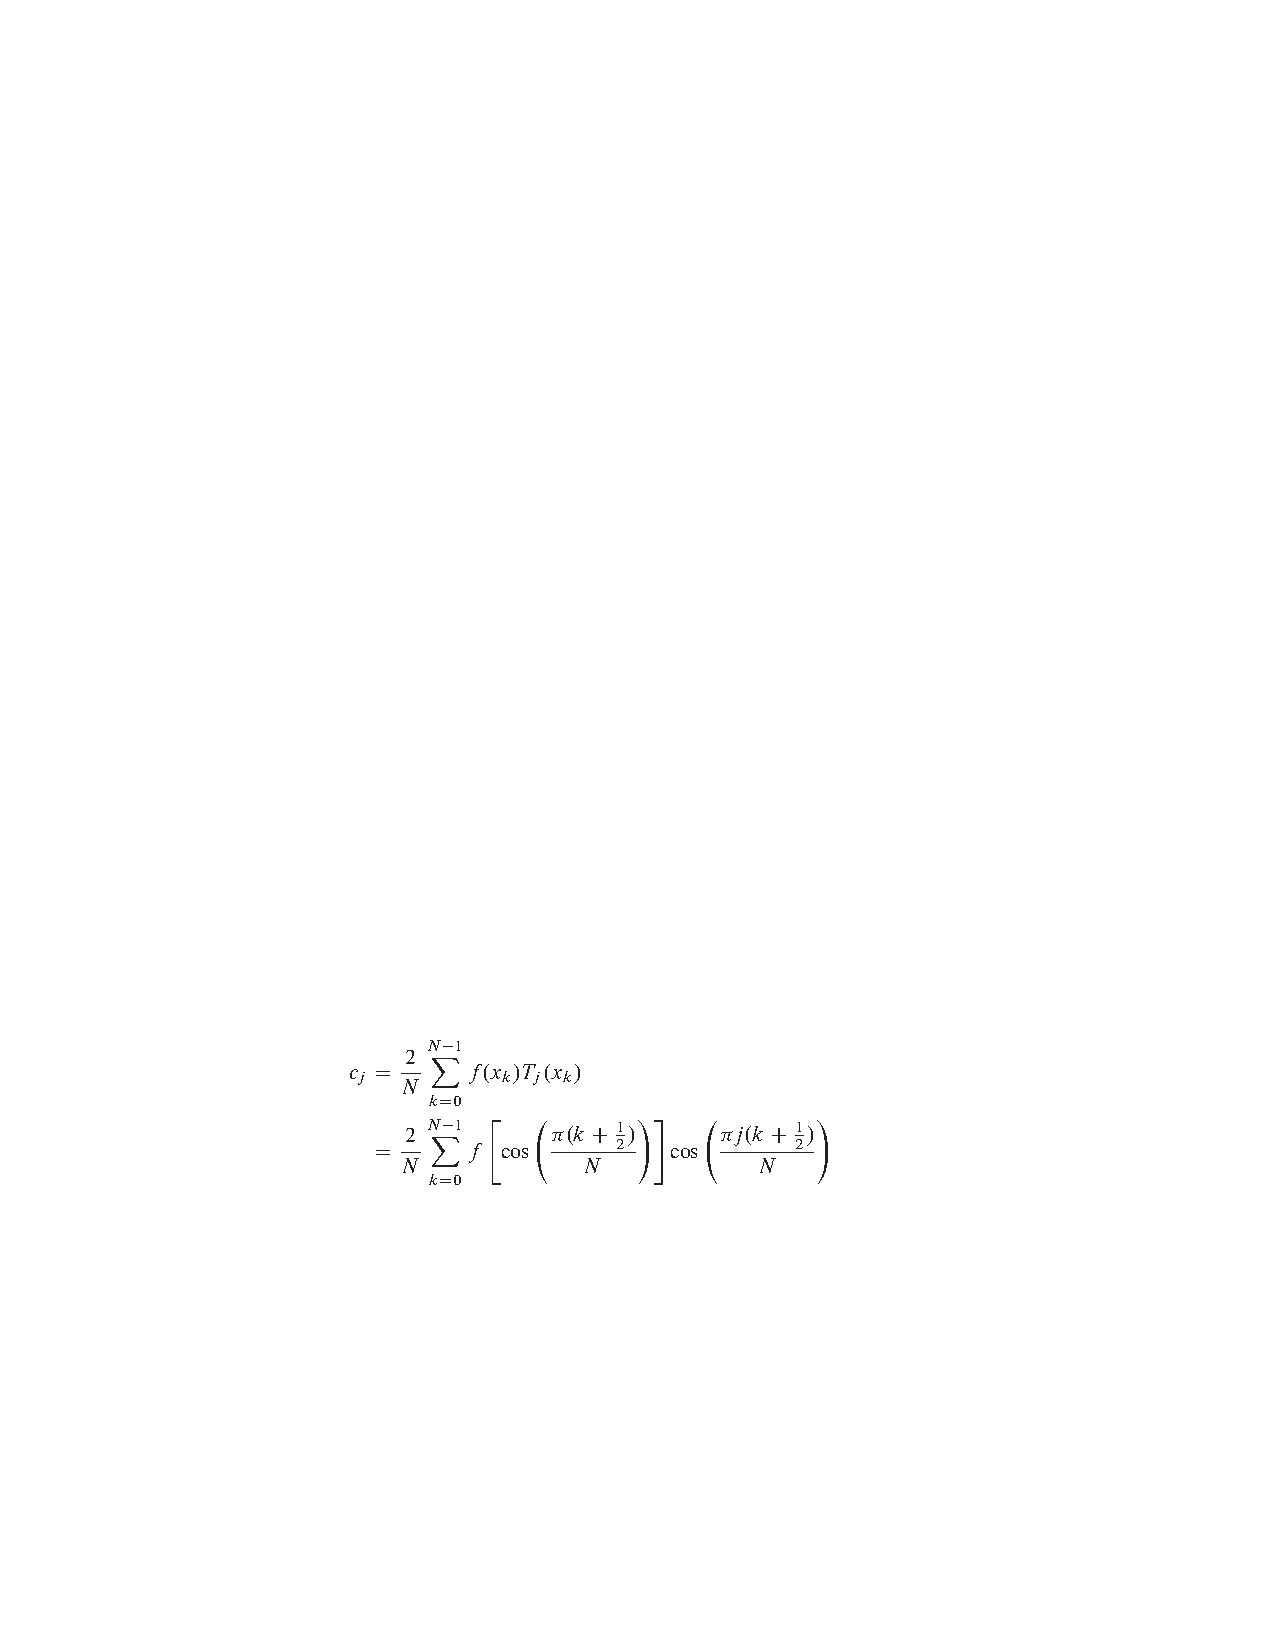
\includegraphics[width=0.8\textwidth]{ChebyCj.pdf}\\
        Function approximation is exponentially accurate in order:\\
        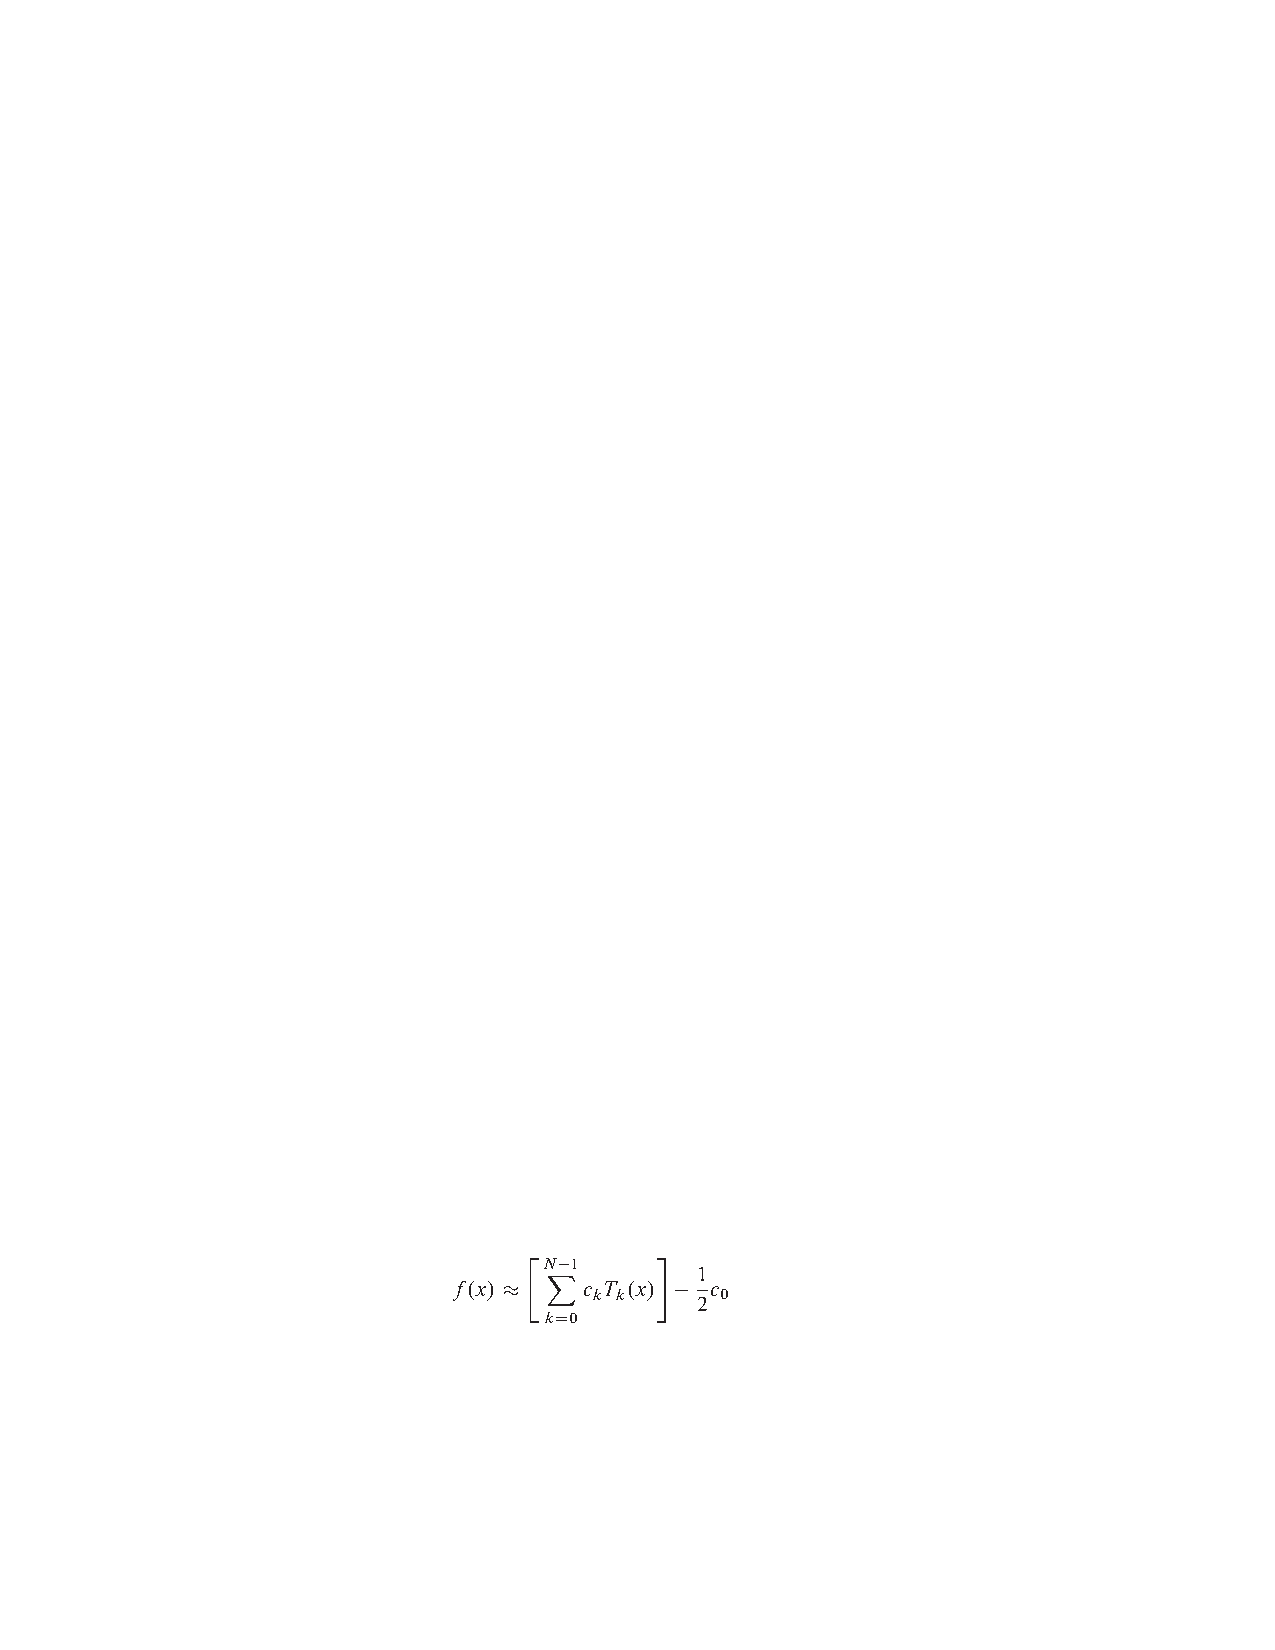
\includegraphics[width=0.5\textwidth]{ChebyApprox.pdf}
      \end{column}
      \begin{column}{0.5\textwidth}
        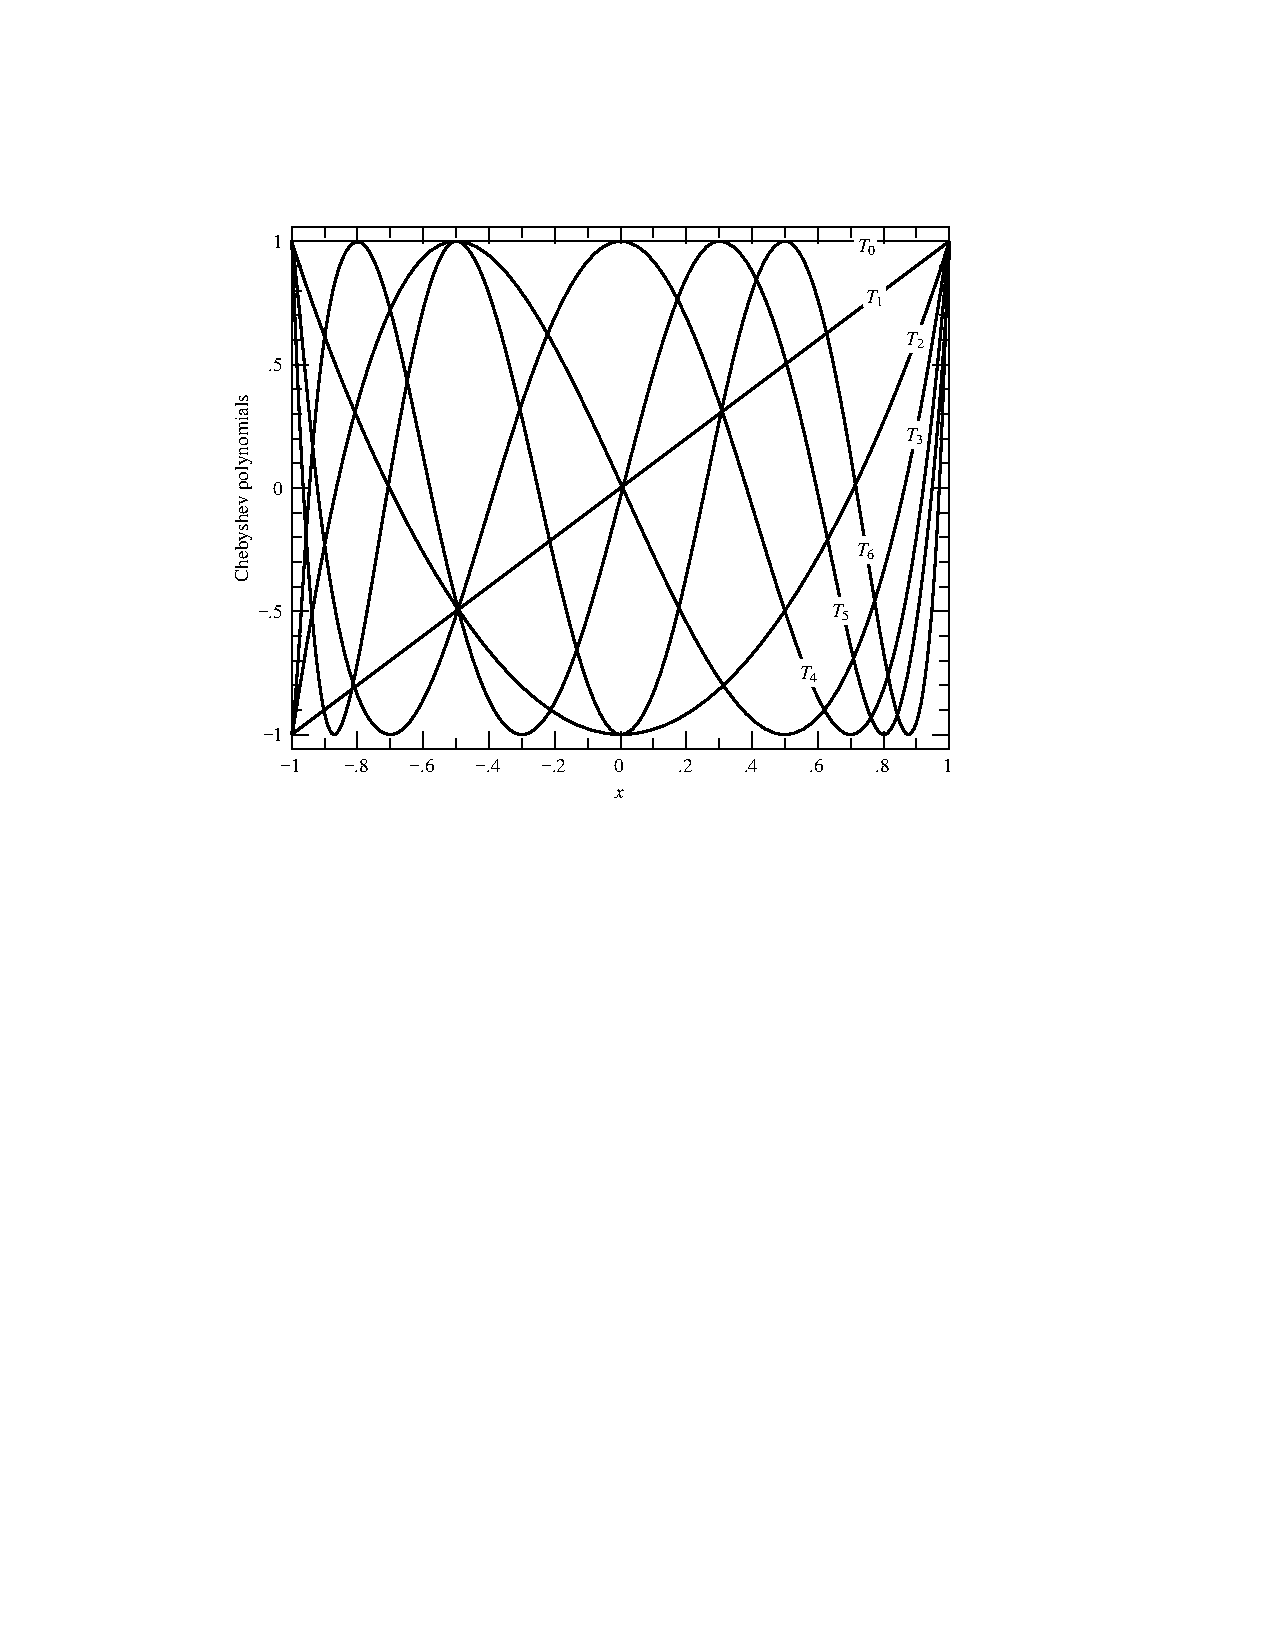
\includegraphics[width=\textwidth]{ChebyOrthog.pdf}
        \begin{itemize}
          \item Special case of $f(x) = \frac{1}{x}$ corresponds to sparse matrix inversion
          \item Could used to solve propagators in LQCD (instead use Krylov solvers)
          \item Apply polynomial of matrix to a \emph{source}
          \item Obtains one row of the inverse matrix
          \item Solving O(volume) times is required for complete inverse - impractical
          \item Never solve linear equations exactly; $10^{11}$ degrees of freedom
          \item $10^{-10}$ is typically sufficient
          \end{itemize}
      \end{column}
      \end{columns}
  \end{frame}


\begin{frame}[fragile]\small\frametitle{ Exercise}

\begin{itemize}
\item Based on example 1, implement covariant Wuppertal smearing with one of the Laplacian operators 
\begin{itemize}
\item Negate the operator, so its eigenvalues are \emph{positive}
\item Apply this to a kronecker delta function at the midpoint of the lattice (pokeSite)
\item Output the smeared field to \verb1 std::cout 1
\item Use grep and gnuplot to plot the profile as a function of $x$ and $y$
\item \verb9 ./Example_Laplacian_smearing --grid 16.16.16.2 | grep ^.*,8,8,0 9
  \end{itemize}
\item Advanced: Use the Grid Chebyshev classes to implement a free $F(p^2)$ smearing and choose a form that gives a radial node
  \begin{itemize}
  \item Congratulations: you've invented a powerful new form of covariant Lattice smearing (!)
\end{itemize}
\item \emph{Only if necessary} peek at
  \href{https://github.com/paboyle/Grid/blob/develop/examples/Example_Laplacian_smearing.cc}{\color{blue}https://github.com/paboyle/Grid/blob/develop/examples/Example\_Laplacian\_smearing.cc}
\item The example solution also implements a form of $\theta(p^2)$ that allows to compare to Distillation smearing
\begin{itemize}
\item Satisfy yourself that Distillation tends to a point operator as the threshold for the $\theta-$function is increased
\end{itemize}
\item Strongly encourage you to \emph{play with codes} coming at things from different directions. \\
  {\bf Everything has to work out as you expect (after a little thought!) or the code is wrong}. \\
  The experience gained will bring invaluable debug skills and more rapid development capability.
\item If it doesn't work in the free field where we know the answers, it won't work in the interacting case!
\end{itemize}

\end{frame}
  
\begin{frame}[fragile]\small\frametitle{ Advanced Exercise}

\begin{itemize}
\item Implement a stencil based adjoint representation Laplacian for SU(3).
\begin{itemize}
\item Check against the slow Cshift implementation: \link{https://github.com/paboyle/Grid/blob/develop/Grid/qcd/utils/CovariantLaplacian.h}
\end{itemize}
\item Send me the code: I promised Chulwoo Jung I would write it (!)
\end{itemize}

\end{frame}


\end{document}



